\pdfoutput=1
%% Author: PGL  Porta Mana
%% Created: 2015-05-01T20:53:34+0200
%% Last-Updated: 2023-02-24T13:26:17+0100
%%%%%%%%%%%%%%%%%%%%%%%%%%%%%%%%%%%%%%%%%%%%%%%%%%%%%%%%%%%%%%%%%%%%%%%%%%%%
\newif\ifarxiv
\arxivfalse
\iftrue\pdfmapfile{+classico.map}\fi
\newif\ifafour
\afourfalse% true = A4, false = A5
\newif\iftypodisclaim % typographical disclaim on the side
\typodisclaimtrue
\newcommand*{\memfontfamily}{zplx}
\newcommand*{\memfontpack}{newpxtext}
\documentclass[\ifafour a4paper,12pt,\else a5paper,10pt,\fi%extrafontsizes,%
onecolumn,oneside,article,%french,italian,german,swedish,latin,
british%
]{memoir}
\newcommand*{\firstdraft}{15 January 2023}
\newcommand*{\firstpublished}{\firstdraft}
\newcommand*{\updated}{\ifarxiv***\else\today\ [draft]\fi}
\newcommand*{\propertitle}{\Large Foundations of inference under symmetry:\\
{\large A derivation of algorithms for non-parametric density inference}% 
}% title uses LARGE; set Large for smaller
\newcommand*{\pdftitle}{\propertitle}
\newcommand*{\headtitle}{}
\newcommand*{\pdfauthor}{M. Koci\'nski, A. Lundervold\, A. J. Lundervold, A. S. Lundervold, P.G.L.  Porta Mana, I. Rye, A.~Vik}
\newcommand*{\headauthor}{Porta Mana \etal}
\newcommand*{\reporthead}{\ifarxiv\else Open Science Framework \href{https://doi.org/10.31219/osf.io/***}{\textsc{doi}:10.31219/osf.io/***}\fi}% Report number

%%%%%%%%%%%%%%%%%%%%%%%%%%%%%%%%%%%%%%%%%%%%%%%%%%%%%%%%%%%%%%%%%%%%%%%%%%%%
%%% Calls to packages (uncomment as needed)
%%%%%%%%%%%%%%%%%%%%%%%%%%%%%%%%%%%%%%%%%%%%%%%%%%%%%%%%%%%%%%%%%%%%%%%%%%%%

%\usepackage{pifont}

%\usepackage{fontawesome}

\usepackage[T1]{fontenc} 
\input{glyphtounicode} \pdfgentounicode=1

\usepackage[utf8]{inputenx}

%\usepackage{newunicodechar}
% \newunicodechar{Ĕ}{\u{E}}
% \newunicodechar{ĕ}{\u{e}}
% \newunicodechar{Ĭ}{\u{I}}
% \newunicodechar{ĭ}{\u{\i}}
% \newunicodechar{Ŏ}{\u{O}}
% \newunicodechar{ŏ}{\u{o}}
% \newunicodechar{Ŭ}{\u{U}}
% \newunicodechar{ŭ}{\u{u}}
% \newunicodechar{Ā}{\=A}
% \newunicodechar{ā}{\=a}
% \newunicodechar{Ē}{\=E}
% \newunicodechar{ē}{\=e}
% \newunicodechar{Ī}{\=I}
% \newunicodechar{ī}{\={\i}}
% \newunicodechar{Ō}{\=O}
% \newunicodechar{ō}{\=o}
% \newunicodechar{Ū}{\=U}
% \newunicodechar{ū}{\=u}
% \newunicodechar{Ȳ}{\=Y}
% \newunicodechar{ȳ}{\=y}

\newcommand*{\bmmax}{0} % reduce number of bold fonts, before font packages
\newcommand*{\hmmax}{0} % reduce number of heavy fonts, before font packages

\usepackage{textcomp}

%\usepackage[normalem]{ulem}% package for underlining
% \makeatletter
% \def\ssout{\bgroup \ULdepth=-.35ex%\UL@setULdepth
%  \markoverwith{\lower\ULdepth\hbox
%    {\kern-.03em\vbox{\hrule width.2em\kern1.2\p@\hrule}\kern-.03em}}%
%  \ULon}
% \makeatother

\usepackage{amsmath}

\usepackage{mathtools}
%\addtolength{\jot}{\jot} % increase spacing in multiline formulae
\setlength{\multlinegap}{0pt}

%\usepackage{empheq}% automatically calls amsmath and mathtools
%\newcommand*{\widefbox}[1]{\fbox{\hspace{1em}#1\hspace{1em}}}

%%%% empheq above seems more versatile than these:
%\usepackage{fancybox}
%\usepackage{framed}

% \usepackage[misc]{ifsym} % for dice
% \newcommand*{\diceone}{{\scriptsize\Cube{1}}}

\usepackage{amssymb}

\usepackage{amsxtra}

\usepackage[main=british]{babel}\selectlanguage{british}
%\newcommand*{\langnohyph}{\foreignlanguage{nohyphenation}}
\newcommand{\langnohyph}[1]{\begin{hyphenrules}{nohyphenation}#1\end{hyphenrules}}

\usepackage[autostyle=false,autopunct=false,english=british]{csquotes}
\setquotestyle{american}
\newcommand*{\defquote}[1]{`\,#1\,'}

% \makeatletter
% \renewenvironment{quotation}%
%                {\list{}{\listparindent 1.5em%
%                         \itemindent    \listparindent
%                         \rightmargin=1em   \leftmargin=1em
%                         \parsep        \z@ \@plus\p@}%
%                 \item[]\footnotesize}%
%                 {\endlist}
% \makeatother                


\usepackage{amsthm}
%% from https://tex.stackexchange.com/a/404680/97039
\makeatletter
\def\@endtheorem{\endtrivlist}
\makeatother

\newcommand*{\QED}{\textsc{q.e.d.}}
\renewcommand*{\qedsymbol}{\QED}
\theoremstyle{remark}
\newtheorem{note}{Note}
\newtheorem*{remark}{Note}
\newtheoremstyle{innote}{\parsep}{\parsep}{\footnotesize}{}{}{}{0pt}{}
\theoremstyle{innote}
\newtheorem*{innote}{}

\usepackage[shortlabels,inline]{enumitem}
\SetEnumitemKey{para}{itemindent=\parindent,leftmargin=0pt,listparindent=\parindent,parsep=0pt,itemsep=\topsep}
% \begin{asparaenum} = \begin{enumerate}[para]
% \begin{inparaenum} = \begin{enumerate*}
\setlist{itemsep=0pt,topsep=\parsep}
\setlist[enumerate,2]{label=(\roman*)}
\setlist[enumerate]{label=(\alph*),leftmargin=1.5\parindent}
\setlist[itemize]{leftmargin=1.5\parindent}
\setlist[description]{leftmargin=1.5\parindent}
% old alternative:
% \setlist[enumerate,2]{label=\alph*.}
% \setlist[enumerate]{leftmargin=\parindent}
% \setlist[itemize]{leftmargin=\parindent}
% \setlist[description]{leftmargin=\parindent}

\usepackage[babel,theoremfont,largesc]{newpxtext}

% For Baskerville see https://ctan.org/tex-archive/fonts/baskervillef?lang=en
% and http://mirrors.ctan.org/fonts/baskervillef/doc/baskervillef-doc.pdf
% \usepackage[p]{baskervillef}
% \usepackage[varqu,varl,var0]{inconsolata}
% \usepackage[scale=.95,type1]{cabin}
% \usepackage[baskerville,vvarbb]{newtxmath}
% \usepackage[cal=boondoxo]{mathalfa}


\usepackage[bigdelims,nosymbolsc%,smallerops % probably arXiv doesn't have it
]{newpxmath}
%\useosf
%\linespread{1.083}%
%\linespread{1.05}% widely used
\linespread{1.1}% best for text with maths
%% smaller operators for old version of newpxmath
\makeatletter
\def\re@DeclareMathSymbol#1#2#3#4{%
    \let#1=\undefined
    \DeclareMathSymbol{#1}{#2}{#3}{#4}}
%\re@DeclareMathSymbol{\bigsqcupop}{\mathop}{largesymbols}{"46}
%\re@DeclareMathSymbol{\bigodotop}{\mathop}{largesymbols}{"4A}
\re@DeclareMathSymbol{\bigoplusop}{\mathop}{largesymbols}{"4C}
\re@DeclareMathSymbol{\bigotimesop}{\mathop}{largesymbols}{"4E}
\re@DeclareMathSymbol{\sumop}{\mathop}{largesymbols}{"50}
\re@DeclareMathSymbol{\prodop}{\mathop}{largesymbols}{"51}
\re@DeclareMathSymbol{\bigcupop}{\mathop}{largesymbols}{"53}
\re@DeclareMathSymbol{\bigcapop}{\mathop}{largesymbols}{"54}
%\re@DeclareMathSymbol{\biguplusop}{\mathop}{largesymbols}{"55}
\re@DeclareMathSymbol{\bigwedgeop}{\mathop}{largesymbols}{"56}
\re@DeclareMathSymbol{\bigveeop}{\mathop}{largesymbols}{"57}
%\re@DeclareMathSymbol{\bigcupdotop}{\mathop}{largesymbols}{"DF}
%\re@DeclareMathSymbol{\bigcapplusop}{\mathop}{largesymbolsPXA}{"00}
%\re@DeclareMathSymbol{\bigsqcupplusop}{\mathop}{largesymbolsPXA}{"02}
%\re@DeclareMathSymbol{\bigsqcapplusop}{\mathop}{largesymbolsPXA}{"04}
%\re@DeclareMathSymbol{\bigsqcapop}{\mathop}{largesymbolsPXA}{"06}
\re@DeclareMathSymbol{\bigtimesop}{\mathop}{largesymbolsPXA}{"10}
%\re@DeclareMathSymbol{\coprodop}{\mathop}{largesymbols}{"60}
%\re@DeclareMathSymbol{\varprod}{\mathop}{largesymbolsPXA}{16}
\makeatother
%%
%% With euler font cursive for Greek letters - the [1] means 100% scaling
\DeclareFontFamily{U}{egreek}{\skewchar\font'177}%
\DeclareFontShape{U}{egreek}{m}{n}{<-6>s*[1]eurm5 <6-8>s*[1]eurm7 <8->s*[1]eurm10}{}%
\DeclareFontShape{U}{egreek}{m}{it}{<->s*[1]eurmo10}{}%
\DeclareFontShape{U}{egreek}{b}{n}{<-6>s*[1]eurb5 <6-8>s*[1]eurb7 <8->s*[1]eurb10}{}%
\DeclareFontShape{U}{egreek}{b}{it}{<->s*[1]eurbo10}{}%
\DeclareSymbolFont{egreeki}{U}{egreek}{m}{it}%
\SetSymbolFont{egreeki}{bold}{U}{egreek}{b}{it}% from the amsfonts package
\DeclareSymbolFont{egreekr}{U}{egreek}{m}{n}%
\SetSymbolFont{egreekr}{bold}{U}{egreek}{b}{n}% from the amsfonts package
% Take also \sum, \prod, \coprod symbols from Euler fonts
\DeclareFontFamily{U}{egreekx}{\skewchar\font'177}
\DeclareFontShape{U}{egreekx}{m}{n}{%
       <-7.5>s*[0.9]euex7%
    <7.5-8.5>s*[0.9]euex8%
    <8.5-9.5>s*[0.9]euex9%
    <9.5->s*[0.9]euex10%
}{}
\DeclareSymbolFont{egreekx}{U}{egreekx}{m}{n}
\DeclareMathSymbol{\sumop}{\mathop}{egreekx}{"50}
\DeclareMathSymbol{\prodop}{\mathop}{egreekx}{"51}
\DeclareMathSymbol{\coprodop}{\mathop}{egreekx}{"60}
\makeatletter
\def\sum{\DOTSI\sumop\slimits@}
\def\prod{\DOTSI\prodop\slimits@}
\def\coprod{\DOTSI\coprodop\slimits@}
\makeatother
% Greek letters not usually given in LaTeX.
\DeclareMathSymbol{\varpartial}{\mathalpha}{egreeki}{"40}
\DeclareMathSymbol{\partialup}{\mathalpha}{egreekr}{"40}
\DeclareMathSymbol{\alpha}{\mathalpha}{egreeki}{"0B}
\DeclareMathSymbol{\beta}{\mathalpha}{egreeki}{"0C}
\DeclareMathSymbol{\gamma}{\mathalpha}{egreeki}{"0D}
\DeclareMathSymbol{\delta}{\mathalpha}{egreeki}{"0E}
\DeclareMathSymbol{\epsilon}{\mathalpha}{egreeki}{"0F}
\DeclareMathSymbol{\zeta}{\mathalpha}{egreeki}{"10}
\DeclareMathSymbol{\eta}{\mathalpha}{egreeki}{"11}
\DeclareMathSymbol{\theta}{\mathalpha}{egreeki}{"12}
\DeclareMathSymbol{\iota}{\mathalpha}{egreeki}{"13}
\DeclareMathSymbol{\kappa}{\mathalpha}{egreeki}{"14}
\DeclareMathSymbol{\lambda}{\mathalpha}{egreeki}{"15}
\DeclareMathSymbol{\mu}{\mathalpha}{egreeki}{"16}
\DeclareMathSymbol{\nu}{\mathalpha}{egreeki}{"17}
\DeclareMathSymbol{\xi}{\mathalpha}{egreeki}{"18}
\DeclareMathSymbol{\omicron}{\mathalpha}{egreeki}{"6F}
\DeclareMathSymbol{\pi}{\mathalpha}{egreeki}{"19}
\DeclareMathSymbol{\rho}{\mathalpha}{egreeki}{"1A}
\DeclareMathSymbol{\sigma}{\mathalpha}{egreeki}{"1B}
 \DeclareMathSymbol{\tau}{\mathalpha}{egreeki}{"1C}
\DeclareMathSymbol{\upsilon}{\mathalpha}{egreeki}{"1D}
\DeclareMathSymbol{\phi}{\mathalpha}{egreeki}{"1E}
\DeclareMathSymbol{\chi}{\mathalpha}{egreeki}{"1F}
\DeclareMathSymbol{\psi}{\mathalpha}{egreeki}{"20}
\DeclareMathSymbol{\omega}{\mathalpha}{egreeki}{"21}
\DeclareMathSymbol{\varepsilon}{\mathalpha}{egreeki}{"22}
\DeclareMathSymbol{\vartheta}{\mathalpha}{egreeki}{"23}
\DeclareMathSymbol{\varpi}{\mathalpha}{egreeki}{"24}
\let\varrho\rho 
\let\varsigma\sigma
 \let\varkappa\kappa
\DeclareMathSymbol{\varphi}{\mathalpha}{egreeki}{"27}
%
\DeclareMathSymbol{\varAlpha}{\mathalpha}{egreeki}{"41}
\DeclareMathSymbol{\varBeta}{\mathalpha}{egreeki}{"42}
\DeclareMathSymbol{\varGamma}{\mathalpha}{egreeki}{"00}
\DeclareMathSymbol{\varDelta}{\mathalpha}{egreeki}{"01}
\DeclareMathSymbol{\varEpsilon}{\mathalpha}{egreeki}{"45}
\DeclareMathSymbol{\varZeta}{\mathalpha}{egreeki}{"5A}
\DeclareMathSymbol{\varEta}{\mathalpha}{egreeki}{"48}
\DeclareMathSymbol{\varTheta}{\mathalpha}{egreeki}{"02}
 \DeclareMathSymbol{\varIota}{\mathalpha}{egreeki}{"49}
\DeclareMathSymbol{\varKappa}{\mathalpha}{egreeki}{"4B}
\DeclareMathSymbol{\varLambda}{\mathalpha}{egreeki}{"03}
\DeclareMathSymbol{\varMu}{\mathalpha}{egreeki}{"4D}
\DeclareMathSymbol{\varNu}{\mathalpha}{egreeki}{"4E}
\DeclareMathSymbol{\varXi}{\mathalpha}{egreeki}{"04}
\DeclareMathSymbol{\varOmicron}{\mathalpha}{egreeki}{"4F}
\DeclareMathSymbol{\varPi}{\mathalpha}{egreeki}{"05}
\DeclareMathSymbol{\varRho}{\mathalpha}{egreeki}{"50}
\DeclareMathSymbol{\varSigma}{\mathalpha}{egreeki}{"06}
\DeclareMathSymbol{\varTau}{\mathalpha}{egreeki}{"54}
\DeclareMathSymbol{\varUpsilon}{\mathalpha}{egreeki}{"07}
\DeclareMathSymbol{\varPhi}{\mathalpha}{egreeki}{"08}
\DeclareMathSymbol{\varChi}{\mathalpha}{egreeki}{"58}
\DeclareMathSymbol{\varPsi}{\mathalpha}{egreeki}{"09}
\DeclareMathSymbol{\varOmega}{\mathalpha}{egreeki}{"0A} 
%
\DeclareMathSymbol{\Alpha}{\mathalpha}{egreekr}{"41}
\DeclareMathSymbol{\Beta}{\mathalpha}{egreekr}{"42}
\DeclareMathSymbol{\Gamma}{\mathalpha}{egreekr}{"00}
\DeclareMathSymbol{\Delta}{\mathalpha}{egreekr}{"01}
\DeclareMathSymbol{\Epsilon}{\mathalpha}{egreekr}{"45}
\DeclareMathSymbol{\Zeta}{\mathalpha}{egreekr}{"5A}
\DeclareMathSymbol{\Eta}{\mathalpha}{egreekr}{"48}
\DeclareMathSymbol{\Theta}{\mathalpha}{egreekr}{"02}
\DeclareMathSymbol{\Iota}{\mathalpha}{egreekr}{"49}
\DeclareMathSymbol{\Kappa}{\mathalpha}{egreekr}{"4B}
\DeclareMathSymbol{\Lambda}{\mathalpha}{egreekr}{"03}
\DeclareMathSymbol{\Mu}{\mathalpha}{egreekr}{"4D}
\DeclareMathSymbol{\Nu}{\mathalpha}{egreekr}{"4E}
\DeclareMathSymbol{\Xi}{\mathalpha}{egreekr}{"04}
\DeclareMathSymbol{\Omicron}{\mathalpha}{egreekr}{"4F}
\DeclareMathSymbol{\Pi}{\mathalpha}{egreekr}{"05}
\DeclareMathSymbol{\Rho}{\mathalpha}{egreekr}{"50}
\DeclareMathSymbol{\Sigma}{\mathalpha}{egreekr}{"06}
\DeclareMathSymbol{\Tau}{\mathalpha}{egreekr}{"54}
\DeclareMathSymbol{\Upsilon}{\mathalpha}{egreekr}{"07}
\DeclareMathSymbol{\Phi}{\mathalpha}{egreekr}{"08}
\DeclareMathSymbol{\Chi}{\mathalpha}{egreekr}{"58}
\DeclareMathSymbol{\Psi}{\mathalpha}{egreekr}{"09}
\DeclareMathSymbol{\Omega}{\mathalpha}{egreekr}{"0A}
%
\DeclareMathSymbol{\alphaup}{\mathalpha}{egreekr}{"0B}
\DeclareMathSymbol{\betaup}{\mathalpha}{egreekr}{"0C}
\DeclareMathSymbol{\gammaup}{\mathalpha}{egreekr}{"0D}
 \DeclareMathSymbol{\deltaup}{\mathalpha}{egreekr}{"0E}
\DeclareMathSymbol{\epsilonup}{\mathalpha}{egreekr}{"0F}
\DeclareMathSymbol{\zetaup}{\mathalpha}{egreekr}{"10}
\DeclareMathSymbol{\etaup}{\mathalpha}{egreekr}{"11}
\DeclareMathSymbol{\thetaup}{\mathalpha}{egreekr}{"12}
\DeclareMathSymbol{\iotaup}{\mathalpha}{egreekr}{"13}
\DeclareMathSymbol{\kappaup}{\mathalpha}{egreekr}{"14}
\DeclareMathSymbol{\lambdaup}{\mathalpha}{egreekr}{"15}
\DeclareMathSymbol{\muup}{\mathalpha}{egreekr}{"16}
\DeclareMathSymbol{\nuup}{\mathalpha}{egreekr}{"17}
\DeclareMathSymbol{\xiup}{\mathalpha}{egreekr}{"18}
\DeclareMathSymbol{\omicronup}{\mathalpha}{egreekr}{"6F}
  \DeclareMathSymbol{\piup}{\mathalpha}{egreekr}{"19}
\DeclareMathSymbol{\rhoup}{\mathalpha}{egreekr}{"1A}
\DeclareMathSymbol{\sigmaup}{\mathalpha}{egreekr}{"1B}
\DeclareMathSymbol{\tauup}{\mathalpha}{egreekr}{"1C}
\DeclareMathSymbol{\upsilonup}{\mathalpha}{egreekr}{"1D}
\DeclareMathSymbol{\phiup}{\mathalpha}{egreekr}{"1E}
\DeclareMathSymbol{\chiup}{\mathalpha}{egreekr}{"1F}
\DeclareMathSymbol{\psiup}{\mathalpha}{egreekr}{"20}
\DeclareMathSymbol{\omegaup}{\mathalpha}{egreekr}{"21}
\DeclareMathSymbol{\varepsilonup}{\mathalpha}{egreekr}{"22}
\DeclareMathSymbol{\varthetaup}{\mathalpha}{egreekr}{"23}
\DeclareMathSymbol{\varpiup}{\mathalpha}{egreekr}{"24}
\let\varrhoup\rhoup 
\let\varsigmaup\sigmaup
\let\varkappaup\kappaup
\DeclareMathSymbol{\varphiup}{\mathalpha}{egreekr}{"27}
% Greek letters not usually given in LaTeX.

%\usepackage%[scaled=0.9]%
%{classico}%  Optima as sans-serif font
\renewcommand\sfdefault{uop}
\DeclareMathAlphabet{\mathsf}  {T1}{\sfdefault}{m}{sl}
\SetMathAlphabet{\mathsf}{bold}{T1}{\sfdefault}{b}{sl}
%\newcommand*{\mathte}[1]{\textbf{\textit{\textsf{#1}}}}
% Upright sans-serif math alphabet
% \DeclareMathAlphabet{\mathsu}  {T1}{\sfdefault}{m}{n}
% \SetMathAlphabet{\mathsu}{bold}{T1}{\sfdefault}{b}{n}

% DejaVu Mono as typewriter text
\usepackage[scaled=0.84]{DejaVuSansMono}

\usepackage{mathdots}

\usepackage[usenames]{xcolor}
% Tol (2012) colour-blind-, print-, screen-friendly colours, alternative scheme; Munsell terminology
\definecolor{bluepurple}{RGB}{68,119,170}
\definecolor{blue}{RGB}{102,204,238}
\definecolor{green}{RGB}{34,136,51}
\definecolor{yellow}{RGB}{204,187,68}
\definecolor{red}{RGB}{238,102,119}
\definecolor{redpurple}{RGB}{170,51,119}
\definecolor{grey}{RGB}{187,187,187}
% Tol (2012) colour-blind-, print-, screen-friendly colours; Munsell terminology
% \definecolor{lbpurple}{RGB}{51,34,136}
% \definecolor{lblue}{RGB}{136,204,238}
% \definecolor{lbgreen}{RGB}{68,170,153}
% \definecolor{lgreen}{RGB}{17,119,51}
% \definecolor{lgyellow}{RGB}{153,153,51}
% \definecolor{lyellow}{RGB}{221,204,119}
% \definecolor{lred}{RGB}{204,102,119}
% \definecolor{lpred}{RGB}{136,34,85}
% \definecolor{lrpurple}{RGB}{170,68,153}
\definecolor{lgrey}{RGB}{221,221,221}
%\newcommand*\mycolourbox[1]{%
%\colorbox{grey}{\hspace{1em}#1\hspace{1em}}}
\colorlet{shadecolor}{lgrey}

\usepackage{bm}

\usepackage{microtype}

\usepackage[backend=biber,mcite,%subentry,
citestyle=authoryear-comp,bibstyle=pglpm-authoryear,autopunct=false,sorting=ny,sortcites=false,natbib=false,maxcitenames=2,maxbibnames=8,minbibnames=8,giveninits=true,uniquename=false,uniquelist=false,maxalphanames=1,block=space,hyperref=true,defernumbers=false,useprefix=true,sortupper=false,language=british,parentracker=false,autocite=footnote]{biblatex}
\DeclareSortingTemplate{ny}{\sort{\field{sortname}\field{author}\field{editor}}\sort{\field{year}}}
\DeclareFieldFormat{postnote}{#1}
\iffalse\makeatletter%%% replace parenthesis with brackets
\newrobustcmd*{\parentexttrack}[1]{%
  \begingroup
  \blx@blxinit
  \blx@setsfcodes
  \blx@bibopenparen#1\blx@bibcloseparen
  \endgroup}
\AtEveryCite{%
  \let\parentext=\parentexttrack%
  \let\bibopenparen=\bibopenbracket%
  \let\bibcloseparen=\bibclosebracket}
\makeatother\fi
\DefineBibliographyExtras{british}{\def\finalandcomma{\addcomma}}
\renewcommand*{\finalnamedelim}{\addspace\amp\space}
% \renewcommand*{\finalnamedelim}{\addcomma\space}
\renewcommand*{\textcitedelim}{\addcomma\space}
% \setcounter{biburlnumpenalty}{1} % to allow url breaks anywhere
% \setcounter{biburlucpenalty}{0}
% \setcounter{biburllcpenalty}{1}
\DeclareDelimFormat{multicitedelim}{\addsemicolon\addspace\space}
\DeclareDelimFormat{compcitedelim}{\addsemicolon\addspace\space}
\DeclareDelimFormat{postnotedelim}{\addspace}
\ifarxiv\else\addbibresource{portamanabib.bib}\fi
\renewcommand{\bibfont}{\footnotesize}
%\appto{\citesetup}{\footnotesize}% smaller font for citations
\defbibheading{bibliography}[\bibname]{\section*{#1}\addcontentsline{toc}{section}{#1}%\markboth{#1}{#1}
}
\newcommand*{\citep}{\footcites}
\newcommand*{\citey}{\footcites}%{\parencites*}
\newcommand*{\ibid}{\unspace\addtocounter{footnote}{-1}\footnotemark{}}
%\renewcommand*{\cite}{\parencite}
%\renewcommand*{\cites}{\parencites}
\providecommand{\href}[2]{#2}
\providecommand{\eprint}[2]{\texttt{\href{#1}{#2}}}
\newcommand*{\amp}{\&}
% \newcommand*{\citein}[2][]{\textnormal{\textcite[#1]{#2}}%\addtocategory{extras}{#2}
% }
\newcommand*{\citein}[2][]{\textnormal{\textcite[#1]{#2}}%\addtocategory{extras}{#2}
}
\newcommand*{\citebi}[2][]{\textcite[#1]{#2}%\addtocategory{extras}{#2}
}
\newcommand*{\subtitleproc}[1]{}
\newcommand*{\chapb}{ch.}
%
%\def\UrlOrds{\do\*\do\-\do\~\do\'\do\"\do\-}%
\def\myUrlOrds{\do\0\do\1\do\2\do\3\do\4\do\5\do\6\do\7\do\8\do\9\do\a\do\b\do\c\do\d\do\e\do\f\do\g\do\h\do\i\do\j\do\k\do\l\do\m\do\n\do\o\do\p\do\q\do\r\do\s\do\t\do\u\do\v\do\w\do\x\do\y\do\z\do\A\do\B\do\C\do\D\do\E\do\F\do\G\do\H\do\I\do\J\do\K\do\L\do\M\do\N\do\O\do\P\do\Q\do\R\do\S\do\T\do\U\do\V\do\W\do\X\do\Y\do\Z}%
\makeatletter
%\g@addto@macro\UrlSpecials{\do={\newline}}
\g@addto@macro{\UrlBreaks}{\myUrlOrds}
\makeatother
\newcommand*{\arxiveprint}[1]{%
arXiv \doi{10.48550/arXiv.#1}%
}
\newcommand*{\mparceprint}[1]{%
\href{http://www.ma.utexas.edu/mp_arc-bin/mpa?yn=#1}{mp\_arc:\allowbreak\nolinkurl{#1}}%
}
\newcommand*{\haleprint}[1]{%
\href{https://hal.archives-ouvertes.fr/#1}{\textsc{hal}:\allowbreak\nolinkurl{#1}}%
}
\newcommand*{\philscieprint}[1]{%
\href{http://philsci-archive.pitt.edu/archive/#1}{PhilSci:\allowbreak\nolinkurl{#1}}%
}
\newcommand*{\doi}[1]{%
\href{https://doi.org/#1}{\textsc{doi}:\allowbreak\nolinkurl{#1}}%
}
\newcommand*{\biorxiveprint}[1]{%
bioRxiv \doi{10.1101/#1}%
}
\newcommand*{\osfeprint}[1]{%
Open Science Framework \doi{10.31219/osf.io/#1}%
}
\newcommand*{\osfproj}[1]{%
Open Science Framework \doi{10.17605/osf.io/#1}%
}

\usepackage{graphicx}

%\usepackage{wrapfig}

%\usepackage{tikz-cd}

\PassOptionsToPackage{hyphens}{url}\usepackage[hypertexnames=false,pdfencoding=unicode,psdextra]{hyperref}

\usepackage[depth=4]{bookmark}
\hypersetup{colorlinks=true,bookmarksnumbered,pdfborder={0 0 0.25},citebordercolor={0.2667 0.4667 0.6667},citecolor=bluepurple,linkbordercolor={0.6667 0.2 0.4667},linkcolor=redpurple,urlbordercolor={0.1333 0.5333 0.2},urlcolor=green,breaklinks=true,pdftitle={\pdftitle},pdfauthor={\pdfauthor}}
% \usepackage[vertfit=local]{breakurl}% only for arXiv
\providecommand*{\urlalt}{\href}

\usepackage[british]{datetime2}
\DTMnewdatestyle{mydate}%
{% definitions
\renewcommand*{\DTMdisplaydate}[4]{%
\number##3\ \DTMenglishmonthname{##2} ##1}%
\renewcommand*{\DTMDisplaydate}{\DTMdisplaydate}%
}
\DTMsetdatestyle{mydate}

%%%%%%%%%%%%%%%%%%%%%%%%%%%%%%%%%%%%%%%%%%%%%%%%%%%%%%%%%%%%%%%%%%%%%%%%%%%%
%%% Layout. I do not know on which kind of paper the reader will print the
%%% paper on (A4? letter? one-sided? double-sided?). So I choose A5, which
%%% provides a good layout for reading on screen and save paper if printed
%%% two pages per sheet. Average length line is 66 characters and page
%%% numbers are centred.
%%%%%%%%%%%%%%%%%%%%%%%%%%%%%%%%%%%%%%%%%%%%%%%%%%%%%%%%%%%%%%%%%%%%%%%%%%%%
\ifafour\setstocksize{297mm}{210mm}%{*}% A4
\else\setstocksize{210mm}{5.5in}%{*}% 210x139.7
\fi
\settrimmedsize{\stockheight}{\stockwidth}{*}
\setlxvchars[\normalfont] %313.3632pt for a 66-characters line
\setxlvchars[\normalfont]
% \setlength{\trimtop}{0pt}
% \setlength{\trimedge}{\stockwidth}
% \addtolength{\trimedge}{-\paperwidth}
%\settrims{0pt}{0pt}
% The length of the normalsize alphabet is 133.05988pt - 10 pt = 26.1408pc
% The length of the normalsize alphabet is 159.6719pt - 12pt = 30.3586pc
% Bringhurst gives 32pc as boundary optimal with 69 ch per line
% The length of the normalsize alphabet is 191.60612pt - 14pt = 35.8634pc
\ifafour\settypeblocksize{*}{32pc}{1.618} % A4
%\setulmargins{*}{*}{1.667}%gives 5/3 margins % 2 or 1.667
\else\settypeblocksize{*}{26pc}{1.618}% nearer to a 66-line newpx and preserves GR
\fi
\setulmargins{*}{*}{1}%gives equal margins
\setlrmargins{*}{*}{*}
\setheadfoot{\onelineskip}{2.5\onelineskip}
\setheaderspaces{*}{2\onelineskip}{*}
\setmarginnotes{2ex}{10mm}{0pt}
\checkandfixthelayout[nearest]
%%% End layout
%% this fixes missing white spaces
%\pdfmapline{+dummy-space <dummy-space.pfb}
%\pdfinterwordspaceon% seems to add a white margin to Sumatrapdf

%%% Sectioning
\newcommand*{\asudedication}[1]{%
{\par\centering\textit{#1}\par}}
\newenvironment{acknowledgements}{\section*{Thanks}\addcontentsline{toc}{section}{Thanks}}{\par}
\makeatletter\renewcommand{\appendix}{\par
  \bigskip{\centering
   \interlinepenalty \@M
   \normalfont
   \printchaptertitle{\sffamily\appendixpagename}\par}
  \setcounter{section}{0}%
  \gdef\@chapapp{\appendixname}%
  \gdef\thesection{\@Alph\c@section}%
  \anappendixtrue}\makeatother
\counterwithout{section}{chapter}
\setsecnumformat{\upshape\csname the#1\endcsname\quad}
\setsecheadstyle{\large\bfseries\sffamily%
\centering}
\setsubsecheadstyle{\bfseries\sffamily%
\raggedright}
%\setbeforesecskip{-1.5ex plus 1ex minus .2ex}% plus 1ex minus .2ex}
%\setaftersecskip{1.3ex plus .2ex }% plus 1ex minus .2ex}
%\setsubsubsecheadstyle{\bfseries\sffamily\slshape\raggedright}
%\setbeforesubsecskip{1.25ex plus 1ex minus .2ex }% plus 1ex minus .2ex}
%\setaftersubsecskip{-1em}%{-0.5ex plus .2ex}% plus 1ex minus .2ex}
\setsubsecindent{0pt}%0ex plus 1ex minus .2ex}
\setparaheadstyle{\bfseries\sffamily%
\raggedright}
\setcounter{secnumdepth}{2}
\setlength{\headwidth}{\textwidth}
\newcommand{\addchap}[1]{\chapter*[#1]{#1}\addcontentsline{toc}{chapter}{#1}}
\newcommand{\addsec}[1]{\section*{#1}\addcontentsline{toc}{section}{#1}}
\newcommand{\addsubsec}[1]{\subsection*{#1}\addcontentsline{toc}{subsection}{#1}}
\newcommand{\addpara}[1]{\paragraph*{#1.}\addcontentsline{toc}{subsubsection}{#1}}
\newcommand{\addparap}[1]{\paragraph*{#1}\addcontentsline{toc}{subsubsection}{#1}}

%%% Headers, footers, pagestyle
\copypagestyle{manaart}{plain}
\makeheadrule{manaart}{\headwidth}{0.5\normalrulethickness}
\makeoddhead{manaart}{%
{\footnotesize%\sffamily%
\scshape\headauthor}}{}{{\footnotesize\sffamily%
\headtitle}}
\makeoddfoot{manaart}{}{\thepage}{}
\newcommand*\autanet{
\includegraphics[height=\heightof{M}]{autanet.pdf}}
\definecolor{mygray}{gray}{0.333}
\iftypodisclaim%
\ifafour\newcommand\addprintnote{\begin{picture}(0,0)%
\put(245,149){\makebox(0,0){\rotatebox{90}{\tiny\color{mygray}\textsf{This
            document is designed for screen reading and
            two-up printing on A4 or Letter paper}}}}%
\end{picture}}% A4
\else\newcommand\addprintnote{\begin{picture}(0,0)%
\put(176,112){\makebox(0,0){\rotatebox{90}{\tiny\color{mygray}\textsf{This
            document is designed for screen reading and
            two-up printing on A4 or Letter paper}}}}%
\end{picture}}\fi%afourtrue
\makeoddfoot{plain}{}{\makebox[0pt]{\thepage}\addprintnote}{}
\else
\makeoddfoot{plain}{}{\makebox[0pt]{\thepage}}{}
\fi%typodisclaimtrue
\makeoddhead{plain}{\scriptsize\reporthead}{}{}
% \copypagestyle{manainitial}{plain}
% \makeheadrule{manainitial}{\headwidth}{0.5\normalrulethickness}
% \makeoddhead{manainitial}{%
% \footnotesize\sffamily%
% \scshape\headauthor}{}{\footnotesize\sffamily%
% \headtitle}
% \makeoddfoot{manaart}{}{\thepage}{}

\pagestyle{manaart}

\setlength{\droptitle}{-3.9\onelineskip}
\pretitle{\begin{center}\LARGE\sffamily%
\bfseries}
\posttitle{\bigskip\end{center}}

\makeatletter\newcommand*{\atf}{
\includegraphics[totalheight=\heightof{@}]{atblack.png}}\makeatother
\providecommand{\affiliation}[1]{\textsl{\textsf{\footnotesize #1}}}
\providecommand{\epost}[1]{\texttt{\footnotesize\textless#1\textgreater}}
\providecommand{\email}[2]{\href{mailto:#1ZZ@#2 ((remove ZZ))}{#1\protect\atf#2}}
%\providecommand{\email}[2]{\href{mailto:#1@#2}{#1@#2}}

\preauthor{\vspace{-0.5\baselineskip}\begin{center}
\normalsize\sffamily%
\lineskip  0.5em}
\postauthor{\par\end{center}}
\predate{\DTMsetdatestyle{mydate}\begin{center}\footnotesize}
\postdate{\end{center}\vspace{-\medskipamount}}

\setfloatadjustment{figure}{\footnotesize}
\captiondelim{\quad}
\captionnamefont{\footnotesize\sffamily%
}
\captiontitlefont{\footnotesize}
%\firmlists*
\midsloppy
% handling orphan/widow lines, memman.pdf
% \clubpenalty=10000
% \widowpenalty=10000
% \raggedbottom
% Downes, memman.pdf
\clubpenalty=9996
\widowpenalty=9999
\brokenpenalty=4991
\predisplaypenalty=10000
\postdisplaypenalty=1549
\displaywidowpenalty=1602
\raggedbottom

\paragraphfootnotes
\setlength{\footmarkwidth}{2ex}
% \threecolumnfootnotes
%\setlength{\footmarksep}{0em}
\footmarkstyle{\textsuperscript{%\color{red}
\scriptsize\bfseries#1}~}
%\footmarkstyle{\textsuperscript{\color{red}\scriptsize\bfseries#1}~}
%\footmarkstyle{\textsuperscript{[#1]}~}

\selectlanguage{british}\frenchspacing

\definecolor{notecolour}{RGB}{68,170,153}
%\newcommand*{\puzzle}{\maltese}
\newcommand*{\puzzle}{{\fontencoding{U}\fontfamily{fontawesometwo}\selectfont\symbol{225}}}
\newcommand*{\wrench}{{\fontencoding{U}\fontfamily{fontawesomethree}\selectfont\symbol{114}}}
\newcommand*{\pencil}{{\fontencoding{U}\fontfamily{fontawesometwo}\selectfont\symbol{210}}}
\newcommand{\mynotew}[1]{{\footnotesize\color{notecolour}\wrench\ #1}}
\newcommand{\mynotep}[1]{{\footnotesize\color{notecolour}\pencil\ #1}}
\newcommand{\mynotez}[1]{{\footnotesize\color{notecolour}\puzzle\ #1}}

%%%%%%%%%%%%%%%%%%%%%%%%%%%%%%%%%%%%%%%%%%%%%%%%%%%%%%%%%%%%%%%%%%%%%%%%%%%%
%%% Paper's details
%%%%%%%%%%%%%%%%%%%%%%%%%%%%%%%%%%%%%%%%%%%%%%%%%%%%%%%%%%%%%%%%%%%%%%%%%%%%
\title{\propertitle}
\author{%
\iffalse\hspace*{\stretch{1}}%
\parbox{0.33\linewidth}%\makebox[0pt][c]%
{\protect\centering M. Koci\'nski %\href{https://orcid.org/0000-0002-6070-0784}{\protect
\includegraphics[scale=0.16]{orcid_32x32.png}}
\\\footnotesize
%Western Norway University of Applied Sciences\quad%
\epost{\email{***}{***}}}%
%%%%%%%%%%%%%%%%%%%%%%%%%%%%%%%%%%%%%%%%%%%%%%%%%%%%%%%%%%%%%%%%%%%%%%%%
\hspace*{\stretch{1}}%
\parbox{0.33\linewidth}%\makebox[0pt][c]%
{\protect\centering A. Lundervold %\href{https://orcid.org/0000-0002-6070-0784}{\protect
\includegraphics[scale=0.16]{orcid_32x32.png}}
\\\footnotesize
%Western Norway University of Applied Sciences\quad%
\epost{\email{***}{***}}}%
%%%%%%%%%%%%%%%%%%%%%%%%%%%%%%%%%%%%%%%%%%%%%%%%%%%%%%%%%%%%%%%%%%%%%%%%
\hspace*{\stretch{1}}%
\parbox{0.33\linewidth}%\makebox[0pt][c]%
{\protect\centering A. J. Lundervold %\href{https://orcid.org/0000-0002-6070-0784}{\protect
\includegraphics[scale=0.16]{orcid_32x32.png}}
\\\footnotesize
%Western Norway University of Applied Sciences\quad%
\epost{\email{***}{***}}}%
%%%%%%%%%%%%%%%%%%%%%%%%%%%%%%%%%%%%%%%%%%%%%%%%%%%%%%%%%%%%%%%%%%%%%%%%
\\\hspace*{\stretch{1}}%
\parbox{0.33\linewidth}%\makebox[0pt][c]%
{\protect\centering A. S. Lundervold %\href{https://orcid.org/0000-0002-6070-0784}{\protect
\includegraphics[scale=0.16]{orcid_32x32.png}}
\\\footnotesize
%Western Norway University of Applied Sciences\quad%
\epost{\email{***}{***}}}%
%%%%%%%%%%%%%%%%%%%%%%%%%%%%%%%%%%%%%%%%%%%%%%%%%%%%%%%%%%%%%%%%%%%%%%%%
\fi\hspace*{\stretch{1}}%
\parbox{0.33\linewidth}%\makebox[0pt][c]%
{\protect\centering P.G.L.  Porta Mana  \href{https://orcid.org/0000-0002-6070-0784}{\protect
\includegraphics[scale=0.16]{orcid_32x32.png}}\\\footnotesize
%Western Norway University of Applied Sciences\quad%
\epost{\email{pgl}{portamana.org}}}%
%%%%%%%%%%%%%%%%%%%%%%%%%%%%%%%%%%%%%%%%%%%%%%%%%%%%%%%%%%%%%%%%%%%%%%%%
\hspace*{\stretch{1}}%
\iffalse\parbox{0.33\linewidth}%\makebox[0pt][c]%
{\protect\centering I. Rye %\href{https://orcid.org/0000-0002-6070-0784}{\protect
\includegraphics[scale=0.16]{orcid_32x32.png}}
\\\footnotesize
%Western Norway University of Applied Sciences\quad%
\epost{\email{***}{***}}}%
%%%%%%%%%%%%%%%%%%%%%%%%%%%%%%%%%%%%%%%%%%%%%%%%%%%%%%%%%%%%%%%%%%%%%%%%
\\\hspace*{\stretch{1}}%
\parbox{0.33\linewidth}%\makebox[0pt][c]%
{\protect\centering A. Vik %\href{https://orcid.org/0000-0002-6070-0784}{\protect
\includegraphics[scale=0.16]{orcid_32x32.png}}
\\\footnotesize
%Western Norway University of Applied Sciences\quad%
\epost{\email{***}{***}}}%
% Mohn Medical Imaging and Visualization Centre, Dept of Computer science, Electrical Engineering and Mathematical Sciences, Western Norway University of Applied Sciences, Bergen, Norway
\hspace*{\stretch{1}}%
\medskip\par{\scriptsize(listed alphabetically)}%
\fi}

%\date{Draft of \today\ (first drafted \firstdraft)}
\date{\firstpublished; updated \updated}

%%%%%%%%%%%%%%%%%%%%%%%%%%%%%%%%%%%%%%%%%%%%%%%%%%%%%%%%%%%%%%%%%%%%%%%%%%%%
%%% Macros @@@
%%%%%%%%%%%%%%%%%%%%%%%%%%%%%%%%%%%%%%%%%%%%%%%%%%%%%%%%%%%%%%%%%%%%%%%%%%%%

% Common ones - uncomment as needed
%\providecommand{\nequiv}{\not\equiv}
%\providecommand{\coloneqq}{\mathrel{\mathop:}=}
%\providecommand{\eqqcolon}{=\mathrel{\mathop:}}
%\providecommand{\varprod}{\prod}
\newcommand*{\de}{\partialup}%partial diff
\newcommand*{\pu}{\piup}%constant pi
\newcommand*{\delt}{\deltaup}%Kronecker, Dirac
%\newcommand*{\eps}{\varepsilonup}%Levi-Civita, Heaviside
%\newcommand*{\riem}{\zetaup}%Riemann zeta
%\providecommand{\degree}{\textdegree}% degree
%\newcommand*{\celsius}{\textcelsius}% degree Celsius
%\newcommand*{\micro}{\textmu}% degree Celsius
% \newcommand*{\I}{\mathrm{i}}%imaginary unit
\newcommand*{\I}{\ensuremath{\mathrm{i}}}
% \newcommand*{\e}{\mathrm{e}}%Neper
\newcommand*{\e}{\ensuremath{\mathrm{e}}}
\newcommand*{\di}{\mathrm{d}}%differential
%% From TUGboat 18 (1997) 1
% \makeatletter
% \providecommand*{\di}%
% {\@ifnextchar^{\DIfF}{\DIfF^{}}}
% \def\DIfF^#1{%
% \mathop{\mathrm{\mathstrut d}}%
% \nolimits^{#1}\gobblespace}
% \def\gobblespace{%
% \futurelet\diffarg\opspace}
% \def\opspace{%
% \let\DiffSpace\!%
% \ifx\diffarg(%
% \let\DiffSpace\relax
% \else
% \ifx\diffarg[%
% \let\DiffSpace\relax
% \else
% \ifx\diffarg\{%
% \let\DiffSpace\relax
% \fi\fi\fi\DiffSpace}
% \makeatother
%\newcommand*{\Di}{\mathrm{D}}%capital differential
%\newcommand*{\Li}{\mathrm{L}}%Lie derivative
%\newcommand*{\planckc}{\hslash}
%\newcommand*{\avogn}{N_{\textrm{A}}}
%\newcommand*{\NN}{\bm{\mathrm{N}}}
%\newcommand*{\ZZ}{\bm{\mathrm{Z}}}
%\newcommand*{\QQ}{\bm{\mathrm{Q}}}
\newcommand*{\RR}{\bm{\mathrm{R}}}
%\newcommand*{\CC}{\bm{\mathrm{C}}}
%\newcommand*{\nabl}{\bm{\nabla}}%nabla
%\DeclareMathOperator{\lb}{lb}%base 2 log
%\DeclareMathOperator{\tr}{tr}%trace
%\DeclareMathOperator{\card}{card}%cardinality
%\DeclareMathOperator{\im}{Im}%im part
%\DeclareMathOperator{\re}{Re}%re part
%\DeclareMathOperator{\sgn}{sgn}%signum
%\DeclareMathOperator{\ent}{ent}%integer less or equal to
%\DeclareMathOperator{\Ord}{O}%same order as
%\DeclareMathOperator{\ord}{o}%lower order than
%\newcommand*{\incr}{\triangle}%finite increment
\newcommand*{\defd}{\coloneqq}
\newcommand*{\defs}{\eqqcolon}
%\newcommand*{\Land}{\bigwedge}
%\newcommand*{\Lor}{\bigvee}
%\newcommand*{\lland}{\DOTSB\;\land\;}
%\newcommand*{\llor}{\DOTSB\;\lor\;}
\newcommand*{\limplies}{\mathbin{\Rightarrow}}%implies
%\newcommand*{\suchthat}{\mid}%{\mathpunct{|}}%such that (eg in sets)
%\newcommand*{\with}{\colon}%with (list of indices)
%\newcommand*{\mul}{\times}%multiplication
%\newcommand*{\inn}{\cdot}%inner product
\newcommand*{\dotv}{\mathord{\,\cdot\,}}%variable place
%\newcommand*{\comp}{\circ}%composition of functions
%\newcommand*{\con}{\mathbin{:}}%scal prod of tensors
%\newcommand*{\equi}{\sim}%equivalent to 
\renewcommand*{\asymp}{\simeq}%equivalent to 
\newcommand*{\corr}{\mathrel{\hat{=}}}%corresponds to
%\providecommand{\varparallel}{\ensuremath{\mathbin{/\mkern-7mu/}}}%parallel (tentative symbol)
\renewcommand*{\le}{\leqslant}%less or equal
\renewcommand*{\ge}{\geqslant}%greater or equal
\DeclarePairedDelimiter\clcl{[}{]}
\DeclarePairedDelimiter\clop{[}{[}
\DeclarePairedDelimiter\opcl{]}{]}
\DeclarePairedDelimiter\opop{]}{[}%}
\DeclarePairedDelimiter\abs{\lvert}{\rvert}
%\DeclarePairedDelimiter\norm{\lVert}{\rVert}
\DeclarePairedDelimiter\set{\{}{\}} %}
%\DeclareMathOperator{\pr}{P}%probability
\newcommand*{\p}{\mathrm{p}}%probability
\renewcommand*{\P}{\mathrm{P}}%probability
\newcommand*{\E}{\mathrm{E}}
%% The "\:" space is chosen to correctly separate inner binary and external rels
\renewcommand*{\|}[1][]{\nonscript\:#1\vert\nonscript\:\mathopen{}}
%\DeclarePairedDelimiterX{\cp}[2]{(}{)}{#1\nonscript\:\delimsize\vert\nonscript\:\mathopen{}#2}
%\DeclarePairedDelimiterX{\ct}[2]{[}{]}{#1\nonscript\;\delimsize\vert\nonscript\:\mathopen{}#2}
%\DeclarePairedDelimiterX{\cs}[2]{\{}{\}}{#1\nonscript\:\delimsize\vert\nonscript\:\mathopen{}#2}
%\newcommand*{\+}{\lor}
%\renewcommand{\*}{\land}
%% symbol = for equality statements within probabilities
%% from https://tex.stackexchange.com/a/484142/97039
% \newcommand*{\eq}{\mathrel{\!=\!}}
% \let\texteq\=
% \renewcommand*{\=}{\TextOrMath\texteq\eq}
% \newcommand*{\eq}[1][=]{\mathrel{\!#1\!}}
\newcommand*{\mo}[1][=]{\mathord{\,#1\,}}
%%
\newcommand*{\sect}{\S}% Sect.~
\newcommand*{\sects}{\S\S}% Sect.~
\newcommand*{\chap}{ch.}%
\newcommand*{\chaps}{chs}%
\newcommand*{\bref}{ref.}%
\newcommand*{\brefs}{refs}%
%\newcommand*{\fn}{fn}%
\newcommand*{\eqn}{eq.}%
\newcommand*{\eqns}{eqs}%
\newcommand*{\fig}{fig.}%
\newcommand*{\figs}{figs}%
\newcommand*{\vs}{{vs}}
\newcommand*{\eg}{{e.g.}}
\newcommand*{\etc}{{etc.}}
\newcommand*{\ie}{{i.e.}}
%\newcommand*{\ca}{{c.}}
\newcommand*{\foll}{{ff.}}
%\newcommand*{\viz}{{viz}}
\newcommand*{\cf}{{cf.}}
%\newcommand*{\Cf}{{Cf.}}
%\newcommand*{\vd}{{v.}}
\newcommand*{\etal}{{et al.}}
%\newcommand*{\etsim}{{et sim.}}
%\newcommand*{\ibid}{{ibid.}}
%\newcommand*{\sic}{{sic}}
%\newcommand*{\id}{\mathte{I}}%id matrix
%\newcommand*{\nbd}{\nobreakdash}%
%\newcommand*{\bd}{\hspace{0pt}}%
%\def\hy{-\penalty0\hskip0pt\relax}
%\newcommand*{\labelbis}[1]{\tag*{(\ref{#1})$_\text{r}$}}
%\newcommand*{\mathbox}[2][.8]{\parbox[t]{#1\columnwidth}{#2}}
%\newcommand*{\zerob}[1]{\makebox[0pt][l]{#1}}
\newcommand*{\tprod}{\mathop{\textstyle\prod}\nolimits}
\newcommand*{\tsum}{\mathop{\textstyle\sum}\nolimits}
%\newcommand*{\tint}{\begingroup\textstyle\int\endgroup\nolimits}
%\newcommand*{\tland}{\mathop{\textstyle\bigwedge}\nolimits}
%\newcommand*{\tlor}{\mathop{\textstyle\bigvee}\nolimits}
%\newcommand*{\sprod}{\mathop{\textstyle\prod}}
%\newcommand*{\ssum}{\mathop{\textstyle\sum}}
%\newcommand*{\sint}{\begingroup\textstyle\int\endgroup}
%\newcommand*{\sland}{\mathop{\textstyle\bigwedge}}
%\newcommand*{\slor}{\mathop{\textstyle\bigvee}}
%\newcommand*{\T}{^\transp}%transpose
%%\newcommand*{\QEM}%{\textnormal{$\Box$}}%{\ding{167}}
%\newcommand*{\qem}{\leavevmode\unskip\penalty9999 \hbox{}\nobreak\hfill
%\quad\hbox{\QEM}}

%%%%%%%%%%%%%%%%%%%%%%%%%%%%%%%%%%%%%%%%%%%%%%%%%%%%%%%%%%%%%%%%%%%%%%%%%%%%
%%% Custom macros for this file @@@
%%%%%%%%%%%%%%%%%%%%%%%%%%%%%%%%%%%%%%%%%%%%%%%%%%%%%%%%%%%%%%%%%%%%%%%%%%%%

\newcommand*{\widebar}[1]{{\mkern1.5mu\skew{2}\overline{\mkern-1.5mu#1\mkern-1.5mu}\mkern 1.5mu}}

% \newcommand{\explanation}[4][t]{%\setlength{\tabcolsep}{-1ex}
% %\smash{
% \begin{tabular}[#1]{c}#2\\[0.5\jot]\rule{1pt}{#3}\\#4\end{tabular}}%}
\newcommand*{\prop}[1]{\enquote{\textsf{#1}}}% for propositions
%\DeclareMathOperator*{\argsup}{arg\,sup}
\newcommand*{\dob}{degree of belief}
\newcommand*{\dobs}{degrees of belief}
\newcommand*{\Iyx}{I}
\newcommand*{\Ix}{I_{\textrm{x}}}
\newcommand*{\Iy}{I_{\textrm{y}}}
\newcommand*{\muo}{\bar{\mu}}
\newcommand*{\sigmao}{\bar{\sigma}}
%%% Custom macros end @@@

%%%%%%%%%%%%%%%%%%%%%%%%%%%%%%%%%%%%%%%%%%%%%%%%%%%%%%%%%%%%%%%%%%%%%%%%%%%%
%%% Beginning of document
%%%%%%%%%%%%%%%%%%%%%%%%%%%%%%%%%%%%%%%%%%%%%%%%%%%%%%%%%%%%%%%%%%%%%%%%%%%%
%\firmlists
\begin{document}
\captiondelim{\quad}\captionnamefont{\footnotesize}\captiontitlefont{\footnotesize}
\selectlanguage{british}\frenchspacing
\maketitle

%%%%%%%%%%%%%%%%%%%%%%%%%%%%%%%%%%%%%%%%%%%%%%%%%%%%%%%%%%%%%%%%%%%%%%%%%%%%
%%% Abstract
%%%%%%%%%%%%%%%%%%%%%%%%%%%%%%%%%%%%%%%%%%%%%%%%%%%%%%%%%%%%%%%%%%%%%%%%%%%%
\abstractrunin
\abslabeldelim{}
\renewcommand*{\abstractname}{}
\setlength{\absleftindent}{0pt}
\setlength{\absrightindent}{0pt}
\setlength{\abstitleskip}{-\absparindent}
\begin{abstract}\labelsep 0pt%
  \noindent ***
% \\\noindent\emph{\footnotesize Note: Dear Reader
%     \amp\ Peer, this manuscript is being peer-reviewed by you. Thank you.}
% \par%\\[\jot]
% \noindent
% {\footnotesize PACS: ***}\qquad%
% {\footnotesize MSC: ***}%
%\qquad{\footnotesize Keywords: ***}
\end{abstract}
\selectlanguage{british}\frenchspacing

%%%%%%%%%%%%%%%%%%%%%%%%%%%%%%%%%%%%%%%%%%%%%%%%%%%%%%%%%%%%%%%%%%%%%%%%%%%%
%%% Epigraph
%%%%%%%%%%%%%%%%%%%%%%%%%%%%%%%%%%%%%%%%%%%%%%%%%%%%%%%%%%%%%%%%%%%%%%%%%%%%
% \asudedication{\small ***}
% \vspace{\bigskipamount}
% \setlength{\epigraphwidth}{.7\columnwidth}
% %\epigraphposition{flushright}
% \epigraphtextposition{flushright}
% %\epigraphsourceposition{flushright}
% \epigraphfontsize{\footnotesize}
% \setlength{\epigraphrule}{0pt}
% %\setlength{\beforeepigraphskip}{0pt}
% %\setlength{\afterepigraphskip}{0pt}
% \epigraph{\emph{text}}{source}



%%%%%%%%%%%%%%%%%%%%%%%%%%%%%%%%%%%%%%%%%%%%%%%%%%%%%%%%%%%%%%%%%%%%%%%%%%%%
%%% BEGINNING OF MAIN TEXT
%%%%%%%%%%%%%%%%%%%%%%%%%%%%%%%%%%%%%%%%%%%%%%%%%%%%%%%%%%%%%%%%%%%%%%%%%%%%

\setcounter{section}{-1}
\section{A warning on notation}
\label{sec:intro}

The probability calculus, being a generalization of the propositional truth-calculus, concerns propositions or statements. In the expression \enquote{$\P(A \| B)$}, $A$ and $B$ thus stand for statements or compositions of statements. In scientific applications most statements of interest are of the form \prop{Measurement of the quantity $X$ yields outcome $x$} or \prop{The quantity $X$ is set to the value $x$}, implicitly or explicitly accompanied by other statements expressing contextual information, for instance \prop{The measurement is made at time~\textellipsis\ in laboratory~\textellipsis\ under conditions~\textellipsis}.

Writing full statements such as these within probability formulae would take an impractical amount of space. This impracticality is solved by an abuse of notation: outside a probability formula, a symbol like $X$ may denote a quantity; but within a probability formula, say $\p(X \| \dotso)$, it instead denotes a full statement such as \prop{Measurement of the quantity $X$ yields outcome $x$}; sometimes the latter is written \prop{$X\mo x$} when the value $x$ is not generic or needs to be explicit.

To limit the confusion that can arise from this notation abuse, I use a convention similar to Jaynes's \parencites*[\sect\,2.5 p.~43]{jaynes1994_r2003}: the probability symbol \enquote{$\P$} is only used when the symbols in its arguments univocally denote statements; the symbol \enquote{$\p$} is used instead to warn that some of the symbols in its arguments are abused. For example, if the quantity $N$ denotes the number of people satisfying some condition, $A\defd{}$\prop{Measurement of $N$ yields $101$ people}, and $B$ denotes some contextual statement, then these three expressions have the same meaning:
\begin{equation*}
  \P(A\|B) = 0.3 \ , \qquad
  \p(N \| B) = 0.3 \ ,\qquad
  \p(N\mo 101 \| B) = 0.3 \ .
\end{equation*}

We take the logical connectives $\lnot$ (not), $\lor$ (or), $\land$ (and) as a functionally complete (redundant) base set. A comma \enquote{,} is interchangeably used for $\land$ in probability formulae. The probability-calculus rules for the base connectives are
\begin{equation}
  \begin{gathered}
% \P(A\|A \land H) = 1
% \qquad
\P(\lnot A\|H) + \P(A \|H) = 1
\\
\P(A\land B \|H) - \P(A\|B\land H) \, \P(B\| H)= 0
  \\
  \P(A\lor B \|H) + \P(A\land B \|H) -\P(A\|H)-  \P(B\| H)=0
  \\
  \text{for any atomic or composite statements $A,B,H$.}
\end{gathered}
\tag{0}\label{eq:Prules}
\end{equation}
The rules ca be used in different guises, for example
\begin{equation*}
  \begin{gathered}
    \textstyle
    \frac{\P(A\|H) = x}{\P(\lnot A \|H) = 1-x}
  \\[\jot]
    \textstyle
  \frac{\P(\lnot A\|H) = x}{\P(A \|H) = 1-x}
\end{gathered}\qquad
  \begin{gathered}
  \textstyle
  \frac{\P(A\|B\land H) = x \quad \P(B\| H)=y}{\P(A\land B \|H) = x y}
  \\[\jot]
  \textstyle
 \frac{\P(A\|B\land H) = x \quad \P(A\land B \|H)=y}{\P(B\| H)=y/x}
\\[\jot]
  \textstyle
 \frac{\P(B\| H) = x \quad \P(A\land B \|H)=y}{\P(A\| B\land H)=y/x}
\end{gathered}\qquad
  \begin{gathered}
\textstyle
  \frac{\P(A\|H) = x \quad \P(B\| H)=y \quad
  \P(A\land B \|H)=z}{\P(A\lor B \|H) = x+y-z}
\\[\jot]
\textstyle
  \frac{\P(A\|H) = x \quad \P(B\| H)=y \quad
  \P(A\lor B \|H)=z}{\P(A\land B \|H) = x+y-z}
\\[\jot]
\textstyle
  \frac{\P(A\|H) = x \quad \P(A\land B \|H) = y\quad 
  \P(A\lor B \|H)=z }{\P(B\| H)=y+z-x}
\end{gathered}
\end{equation*}
Compare with the inference rules for sequent calculi.\autocites[\eg][\chap~1]{huthetal2000_r2004}[App.~A]{prawitz1965}[see also][]{boricic2020}

\section{Inference problem}
\label{sec:inference}

The general context of our inference problem is the following. There is a collection of \enquote{units}, each of which has an associated set of measurable quantities $X_{1},X_{2},\dotsc,Y_{1},Y_{2},\dotsc$, which we call \enquote{variates} according to statistics terminology. The collection of variates $X_{1},X_{2},\dotsc$ is denoted $X$, and similarly for $Y$. % For one or more units we would like to infer the value of some of these variates, say $Y_{1},Y_{2},\dotsc$, given:
% \begin{enumerate*}[label=(\alph*)]
% \item knowledge of some of the remaining ones $X_{1},X_{2},\dotsc$; \item knowledge of some of these variates for other units; \item possibly some additional knowledge specific to the units of interest.
% \end{enumerate*}
Examples: These \enquote{units} could be mechanical gadgets coming out of a production line; the $X$ variates, some of their mechanical properties; the $Y$ variates, other hidden properties or future events such as mechanical failure. Or the units could be clinical patients; the $X$ variates, outcomes of clinical tests performed on these patients; the $Y$ variates, medical conditions or future events such as life length or occurrence of some disease. Our inference context is thus quite general indeed. The units can be labelled with some index $i$, but the values of this index and their ordering have no informational relevance. The variate $X_{1}$ specific to unit $i$ is denoted by $X^{i}_{1}$, and similarly for the other variates.

Our general goal is to make inferences about some of the variates for some of the units, given knowledge about other variates units.

One specific and frequently occurring inference is about the values of the variates $Y^{0}$ for some unit, call it $i=0$, given:
\begin{itemize}%[label=(\alph*)]
\item the values of the variates $X^{0}$ for the same unit; \item the values of the $X,Y$ variates for other units $i=1,2,\dotsc$; \item some auxiliary information $I^{0}$ for the unit $0$; \item all remaining relevant information, denoted $I$.
\end{itemize}

The most general inference gives probabilities to the possible values of $Y^{0}$. Completely certain inference (deduction) is included as a special case with 0 or 1 probabilities.

Thus in mathematical notation we want to determine the distribution of probability
\begin{equation}
  \label{eq:general_prob}
  \p(Y^{0} \| X^{0},\: Y^{1},X^{1},Y^{2},X^{2},\dotsc,\: I^{0},I)
\end{equation}
over the possible values of $Y^{0}$ (more precisely, over statements such as \prop{Measurement of $Y$ for unit $0$ yields $y$}).

Variations of this specific inference are also of interest. For instance, some of the $X$ or $Y$ variate values maybe be unknown for some units; or we want to infer about more than one unit; and similar variations. In the following we show the steps to specifically calculate the probabilities~\eqref{eq:general_prob}; variations of this calculation will be discussed later.

\section{Initial probabilities}
\label{sec:initial_probs}

The propositional truth-calculus allows us to calculate the truth-values of non-tautological statements only if we give the truth-values of some other, related, non-tautological statements, usually called \enquote{premises}. Likewise, the probability calculus allows us to calculate probability-values of non-tautological statements only if we give the probability-values of some other, related, non-tautological statements. These are usually called \enquote{prior} or \enquote{initial} probabilities (these adjectives do \emph{not} imply that these probabilities concern statements about chronologically earlier events).

Therefore we must first assign the probability values of some statements which can lead us to the probabilities~\eqref{eq:general_prob} through the rules~\eqref{eq:Prules}.

There are several prior-probability assignments appropriate to our inference problem. All of them express observations of informational symmetry. Their analysis goes under the name of \enquote{exchangeability} \autocites[For a detailed account with references see][]{bernardoetal1994_r2000}[for a shorter summary,][]{dawid2013}[important references and variations are in][(Appendix on eduction)]{johnson1924}[\sects~4.2--4.3]{johnson1932c}{definetti1930,definetti1937,hewittetal1955,ericson1969,heathetal1976,diaconis1977,diaconisetal1980,diaconisetal1980b,lindleyetal1981}[especially around \sects~7.3, 8.6]{lindley2006_r2014}. Let us start with the most important.

\medskip

Consider the set of units $i=1,2,\dotsc$, excluding $i=0$
According to our information $I$, we have no reason a priori to assign special probabilities to particular units, before we know their variate values $Y^{1},X^{1},Y^{2},X^{2},\dotsc$. This is reflected in the irrelevance of any possible permutation of their indices. This informational symmetry is expressed by the equality of all joint probabilities for sets of values that can be obtained from one another by permutations of the index $i$:
\begin{multline}
  \label{eq:exchang12}
  \p(Y^{1}\mo y^{1},X^{1}\mo x^{1},\ 
  Y^{2}\mo y^{2},X^{2}\mo x^{2},\ 
  Y^{3}\mo y^{3},X^{3}\mo x^{3},\dotsc
  \|I) =
  {}\\
\shoveright{  \p(Y^{1}\mo y^{r(1)},X^{1}\mo x^{r(1)},\ 
  Y^{2}\mo y^{r(2)},X^{2}\mo x^{r(2)},\ 
  Y^{3}\mo y^{r(3)},X^{3}\mo x^{r(3)},\dotsc
  \|I)
}  \\
  \text{for all permutations $r$ and all allowed values $y,x$.}
\end{multline}

If the number of units is large enough, de~Finetti's theorem\ibid\ proves that such a joint probability distribution must then have the following mathematical form:
\begin{multline}
  \label{eq:deFinetti_integral}
  \p(Y^{1}\mo y^{1},X^{1}\mo x^{1},\ 
  Y^{2}\mo y^{2},X^{2}\mo x^{2},\dotsc
  \|I) =
  {}\\
  \int
  F(y^{1},x^{1})\, F(y^{2},x^{2})\,\dotsm
\ \p(\di F \|I)
\end{multline}
the integral being over all normalized, positive weight distributions $F(y,x)$ over the variables $y,x$. The term $\p(\di F \|I)$ is a positive measure over such distributions.

This mathematical representation has an intuitive interpretation. The weight distribution $F(y,x)$ can be interpreted as the frequency distribution of the values $y,x$ among all units. If we knew this frequency distribution, then by symmetry we would assign the probability $F(y,x)$ to measuring $y,x$ on an unsystematically chosen unit, exactly as in sampling from an urn \autocites[\chap~3]{jaynes1994_r2003}. Observations on further units would have probabilities according to \enquote{sampling without replacement}; however, if the total number of units is large and the observed units are few, these probabilities would approximately equal those for \enquote{sampling with replacement} \autocites{heathetal1976}[for error bounds see][]{diaconisetal1980}. These probabilities correspond to the term $F(y^{1},x^{1})\, F(y^{2},x^{2})\,\dotsm$ in the integral. If the frequency distribution $F$ is unknown and we assign a probability density $\p(\di F\|I)$ to it, then the resulting probability for the observations is a convex mixture of the sampling-with-replacement probabilities, weighted by this probability density. This last step follows from the law of total probability, a consequence of the rules~\eqref{eq:Prules}. The integral above corresponds to this convex mixture.

The symmetry or \enquote{exchangeability} requirement does not determine specific numeric values for the joint probability~\eqref{eq:deFinetti_integral}, but greatly restrict our freedom in assigning such values. The only freedom we have left is in the specification of the density $\p(\di F \|I)$. This specification will depend on the particular inference problem and on the nature of the units and variates. The intuitive interpretation of $\p(\di F \|I)$ as our uncertainty about the \enquote{long-run frequencies} can greatly help in this specification. De~Finetti's theorem has moreover an important consequence in this respect: as the values of more and more units become available, the initial numerical choice of density $\p(\di F \|I)$ affects further inferences less and less. Let us discuss these further inferences.

Once the joint probability distribution~\eqref{eq:deFinetti_integral} has been numerically assigned, through specification of $\p(\di F \|I)$, all other marginal and conditional distributions concerning units and variates are also numerically fully determined by repeated application of the rules~\eqref{eq:Prules}. Some examples:
\begin{subequations}
    \label{eq:further_infs}
  \begin{align}
    \p(Y^{2}\mo y^{2} \|I) &=
    \int
    \sum_{x}F(y^{2},x)\,\p(\di F \|I) \ ,
    \\[\jot]
    \p(Y^{2}\mo y^{2} \| X^{2}\mo x^{2}, I) &=
    \frac{\int F(y^{2},x^{2})\ \p(\di F \|I)}{
      \int \sum_{x}F(y^{2},x)\ \p(\di F \|I)
    } \ ,
    \\[\jot]
    \p(Y^{2}\mo y^{2} \| X^{1}\mo x^{1}, I) &=
    \frac{\int \sum_{x}F(y^{2},x)\, \sum_{y}F(y,x^{1})\  \p(\di F \|I)}{
      \int \sum_{y}F(y,x^{1})\  \p(\di F \|I)
    } \ .
  \end{align}
\end{subequations}


\section{Inferences about unit $0$}
\label{sec:unit0}

Any inferences about any variates of any units for which the joint probability distribution~\eqref{eq:deFinetti_integral} is defined can now be probabilistically answered.

Let us consider inferences about a unit, with index $i=0$, about which we have some additional information $I^{0}$.

\subsection{Full symmetry}
\label{sec:unit0_full}

If $\Iyx^{0}$ amounts to saying that the symmetry underlying the probabilities~\eqref{eq:deFinetti_integral} also includes unit $0$, then any probabilities are uniquely determined, as in the examples~\eqref{eq:further_infs}. For instance, our main probability~\eqref{eq:general_prob} is given by
\begin{multline}
  \label{eq:general_prob_fullexch}
  \p(Y^{0}\mo y^{0} \|
  X^{0}\mo x^{0},\: Y^{1}\mo y^{1},X^{1}\mo x^{1},\dotsc,\: \Iyx^{0},I)
  =
{}\\[\jot]
  \frac{
    \int F(y^{0},x^{0})\, F(y^{1},x^{1})\,\dotsm\  \p(\di F \|I)
  }{
    \int \sum_{y}F(y,x^{0})\, F(y^{1},x^{1})\,\dotsm\  \p(\di F \|I)
  } \ .
\end{multline}

\subsection{Symmetry conditional on $X$ variates}
\label{sec:unit0_condX}

A more interesting kind of additional information $\Ix^{0}$  amounts to saying that there is an informational symmetry involving unit~$0$ an the other units, but only with regard to the $Y$ variates, and only with units sharing the same values $x^{*}$ of the $X$ variates. Using a different terminology, this would be a symmetry restricted to a subpopulation of units which is defined by particular $X$ values. Mathematically,
\begin{multline}
  \label{eq:exchangpartial}
  \p(Y^{0}\mo y^{0}, Y^{1}\mo y^{1}, Y^{2}\mo y^{2}
  \|
  X^{0}\mo x^{*}, X^{1}\mo x^{*},X^{2}\mo x^{*},
  \dotsc,\  \Ix^{0},I) =
  {}\\
\shoveright{  \p(Y^{0}\mo y^{r(0)}, Y^{1}\mo y^{r(1)}, Y^{2}\mo y^{r(2)}
  \|
  X^{0}\mo x^{*}, X^{1}\mo x^{*},X^{2}\mo x^{*},
  \dotsc,\  \Ix^{0},I)
}
  \\
  \text{for all permutations $r$ and all allowed values $y,x$.}
\end{multline}
If the number of units is large enough, a variant of de~Finetti's theorem \autocites[\sect\,4.6; their presentation is in terms of the integral~\eqref{eq:deFinetti_integral_partialcond}.]{bernardoetal1994_r2000} proves that such a joint probability distribution must then have the following mathematical form:
\begin{subequations}
  \begin{multline}
    \label{eq:deFinetti_integral_partial}
    \p(Y^{0}\mo y^{0}, Y^{1}\mo y^{1}, Y^{2}\mo y^{2}
    \|
    X^{0}\mo x^{*}, X^{1}\mo x^{*},X^{2}\mo x^{*},
    \dotsc,\  \Ix^{0},I) =
    {}\\
    \int
    \frac{F(y^{0},x^{*})}{\sum_{y}F(y,x^{*})}\,
    \frac{F(y^{1},x^{*})}{\sum_{y}F(y,x^{*})}\,
    \frac{F(y^{2},x^{*})}{\sum_{y}F(y,x^{*})}
    \,\dotsm\ \p(\di F \|I) \ .
  \end{multline}

  This representation has an intuitive interpretation similar to~\eqref{eq:deFinetti_integral}; the difference is that a term like $\frac{F(y^{0},x^{*})}{\sum_{y}F(y,x^{*})}$ now corresponds to the long-run \emph{conditional} frequency $F(y^{0} \| x^{*})$. Our conditional probabilities would be equal to these conditional frequencies if they were known. The uncertainty about the latter leads again to a convex mixture of these conditional probabilities, from the rules~\eqref{eq:Prules}. With a change of variables we could represent the joint frequency $F(y,x)$ as the pair of conditional and marginal frequencies $\bigl(F_{Y\|X}(y\|x), F_{X}(x)\bigr)$. The formula above then simplifies, by marginalization over $\di F_{X}$, to
  \begin{multline}
    \label{eq:deFinetti_integral_partialcond}
    \p(Y^{0}\mo y^{0}, Y^{1}\mo y^{1}, Y^{2}\mo y^{2}
    \|
    X^{0}\mo x^{*}, X^{1}\mo x^{*},X^{2}\mo x^{*},
    \dotsc,\  \Ix^{0},I) =
    {}\\
    \int 
    F(y^{0} \|x^{*})\,   F(y^{1} \|x^{*})\,  F(y^{2} \|x^{*})
    \,\dotsm\ \p(\di F_{Y\|X} \|I) \ .
  \end{multline}
\end{subequations}

Under this kind of auxiliary information $\Ix^{0}$, our main probability~\eqref{eq:general_prob} is given by
\begin{multline}
  \label{eq:general_prob_partialexch}
  \p(Y^{0}\mo y^{0} \|
  X^{0}\mo x^{0},\: Y^{1}\mo y^{1},X^{1}\mo x^{1},\dotsc,\: \Ix^{0},I)
  =
{}\\[\jot]
  \frac{
    \int \frac{F(y^{0},x^{0})}{\sum_{y}F(y,x^{0})}\, F(y^{1},x^{1})\,\dotsm\  \p(\di F \|I)
  }{
    \int F(y^{1},x^{1})\,\dotsm\  \p(\di F \|I)
  } \ .
\end{multline}

\subsection{Symmetry conditional on $Y$ variates}
\label{sec:unit0_condY}

Yet another kind of auxiliary information, $\Iy^{0}$, is the one similar to $\Ix^{0}$ but with the variates $X$ and $Y$ swapped; that is, symmetry under permutation of $X$ values for a subpopulation sharing the same $Y$ values. The discussion proceeds analogously to the previous section up to the representation
  \begin{multline}
    \label{eq:deFinetti_integral_partialY}
    \p(X^{0}\mo x^{0}, X^{1}\mo x^{1}, X^{2}\mo x^{2}
    \|
    Y^{0}\mo y^{*}, Y^{1}\mo y^{*},Y^{2}\mo y^{*},
    \dotsc,\  \Iy^{0},I) =
    {}\\
    \int
    \frac{F(x^{0},y^{*})}{\sum_{x}F(x,y^{*})}\,
    \frac{F(x^{1},y^{*})}{\sum_{x}F(x,y^{*})}\,
    \frac{F(x^{2},y^{*})}{\sum_{x}F(x,y^{*})}
    \,\dotsm\ \p(\di F \|I) \ .
  \end{multline}

  In this case, however, the main probability~\eqref{eq:general_prob} is \emph{not} determined by the probability rules once $\p(\di F\|I)$ has been assigned. We arrive at the following relation, where the proportionality constant can be found by normalizing over $Y^{0}$:
\begin{multline}
  \label{eq:relation_exchY}
  \p(Y^{0}\mo y^{0} \|
  X^{0}\mo x^{0},\: Y^{1}\mo y^{1},X^{1}\mo x^{1},\dotsc,\: \Iy^{0},I)
  \propto
{}\\[2\jot]
  \p(Y^{0}\mo y^{0} \|
  Y^{1}\mo y^{1},X^{1}\mo x^{1},\dotsc,\: \Iy^{0},I) \times{}\\
  \frac{
    \int \frac{F(x^{0},y^{0})}{\sum_{x}F(x,y^{0})}\, F(x^{1},y^{1})\,\dotsm\  \p(\di F \|I)
  }{
    \int F(x^{1},y^{1})\,\dotsm\  \p(\di F \|I)
  } \ .
\end{multline}
The probability in the second row, $\p(Y^{0}\mo y^{0} \| Y^{1}\mo y^{1},X^{1}\mo x^{1},\dotsc,\: \Iy^{0},I)$, must still be assigned \autocites{lindleyetal1981}. This assignment depends strongly on the circumstances. In clinical applications, for example, it is typically further assumed that the units $i=1,2,\dotsc$ are irrelevant for this probability:
\begin{equation}
  \label{eq:indepYfromdata}
    \p(Y^{0}\mo y^{0} \|
  Y^{1}\mo y^{1},X^{1}\mo x^{1},\dotsc,\: \Iy^{0},I) =
    \p(Y^{0}\mo y^{0} \| \Iy^{0},I)
\end{equation}
and $\p(Y^{0}\mo y^{0} \| \Iy^{0},I)$ is taken to be equal to a \emph{base rate}\autocites{barhillel1980,jennyetal2018,sprengeretal2021,matthews1996}, through exchangeability arguments analogous to those of \sect\,\ref{sec:unit0} but without $X$ variates and referred to a \emph{different} sets of units having $Y$ variates.

\subsection{Other symmetries}
\label{sec:other_symm}

It is possible to consider also symmetries for only some of the $X$ variates or some of the $Y$ variates or both, with analyses similar to those of the previous subsections. Finally, it is also possible to consider situations with no symmetries; then the theorems based on exchangeability are not available and one have to assign initial probabilities by different arguments.

\subsection{Common mathematical term}
\label{sec:common_term}

In all examples of additional information $I^{0}$ considered above, the resulting expression for our main probability, \eqns~\eqref{eq:general_prob_fullexch}, \eqref{eq:general_prob_partialexch}, \eqref{eq:relation_exchY}, involve an integral containing a common term: the density
\begin{equation}
  \label{eq:common_density}
  \p(\di F \|D,I) \defd
    \frac{
    F(x^{1},y^{1})\,F(x^{2},y^{2})\,\dotsm\  
  }{
   \int F(x^{1},y^{1})\,F(x^{2},y^{2})\,\dotsm\  \p(\di F \|I)
  } \ ,
\end{equation}
where $D$ is the conjunction of all statements \prop{$Y^{i}\mo y^{i}$}, \prop{$X^{i}\mo x^{i}$} for $i=1,2,\dotsc$. Indeed this probability density can be considered as the updated probability for $\di F$, given the information about all units, $D$.

Our next task is to calculate this term.


\section{A specific representation of $F$ and its densities}
\label{sec:repr_density_F}

\subsection{Mathematical representation of $F$}
\label{sec:repr_F_convexsum}


In order to specify the probability densities $\p(\di F \| I)$ and $\p(\di F \| D, I)$ we need a mathematical representation of the possible joint distributions $F(y,x)$ and of their space; from a differential-geometric point of view \autocites[III.A, VII.A]{choquetbruhatetal1977_r1996}, we want a coordinate system on the manifold of distributions $\set{F}$. It would be an advantage if this mathematical representation would also let us easily compute conditional and marginal distributions such as $F(y\| x)$ and $F(x)$, as we need these to calculate our main probability from formulae~\eqref{eq:general_prob_partialexch} or \eqref{eq:indepYfromdata}.

A very clever representation is discussed by \textcites{dunsonetal2011}\autocites[see also][]{bhattacharyaetal2012,rossi2014}; it is an evolution of representations based on Dirichlet-process mixtures \autocites[\eg][]{antoniak1974,ferguson1983,escobaretal1995,muelleretal1996,rasmussen1999}. It expresses a particular $F(y,x)$ as an in-principle infinite convex mixture of products of parametric distributions $K(\dotso \| \dotso)$:
\begin{multline}
  \label{eq:F_repres}
  F(y_{1},y_{2}, \dotsc,\ x_{1}, x_{2}, \dotsc) ={}\\
  \sum_{c} w^{c}\
  K(y_{1} \| \upsilon^{c}_{1})\,  K(y_{2} \| \upsilon^{c}_{1})\, \dotsm\ 
  K(x_{1} \| \xi^{c}_{1})\,  K(x_{2} \| \xi^{c}_{1})\, \dotsm\ 
\end{multline}
where $w\defd (w^{c})$ are normalized weights, and $\upsilon \defd (\upsilon^{c}_{j})$ and $\xi \defd (\xi^{c}_{j})$ are parameters, possibly multidimensional. The functional forms of the distributions $K(y \| \dotso)$, $K(x \| \dotso)$ depend on the nature of the variates $y,x$. For example $K$ could be a Gaussian distribution for a continuous unbounded variate. The choice of the $K$ depends on the properties expected in the distributions $F$ and on computational requirements.

Any $F$ is thus represented by an in-principle infinite tuple of variables:
\begin{equation}
  \label{eq:F_coords}
  F \corr (w, \upsilon, \xi) \equiv (w^{c}, \upsilon^{c}_{j}, \xi^{c}_{j}) \ .
\end{equation}
The relation between the manifolds $\set{F}$ and $\set{(w, \upsilon, \xi)}$ is typically not one-to-one: different tuples of variables can correspond to the same $F$. We can interpret this as a non-regular embedding $\set{F} \to \set{(w, \upsilon, \xi)}$; or as the existence of different coordinate charts on $\set{F}$, with overlapping domains; or as the expression of $F$ through a frame\autocites{balanetal2006}[\chap~8]{heil1998_r2011}[\chap~3]{daubechies1992_r1999}, rather than through a set of basis functions . This is not a problem for us, because a probability density on the manifold $\set{(w, \upsilon, \xi)}$ also defines, by pull-back, a probability density on the manifold $\set{F}$.

The representation~\eqref{eq:F_repres} is extremely convenient because it leads to simple expressions for conditional and marginal frequencies. For instance in can be easily calculated that
\begin{gather}
  \label{eq:Fconditional_example}
  F(y_{1} \| x_{2}) =
  \sum_{c}
  \frac{ w^{c}\ K(x_{2} \| \xi^{c}_{1})}{
   \sum_{c'} w^{c'}\ K(x_{2} \| \xi^{c'}_{1})
}\ 
  K(y_{1} \| \upsilon^{c}_{1}) \ ,
\\[\jot]
  F(y_{1}) =
  \sum_{c} w^{c}\ K(y_{1} \| \upsilon^{c}_{1}) \ .
\end{gather}

Although the sum in the representation~\eqref{eq:F_repres} is in principle infinite, a particular choice of density for the $(w,\upsilon,\xi)$ variables allows us to approximate it with a finite number of terms, as shown by \textcites{ishwaranetal2002b}. This possibility is essential for computational purposes.

% \medskip

% The representation~\eqref{eq:F_repres} can in turn be embedded in a larger space; this may be convenient for computing the posterior density $\p(\di F \| D,I)$ of \eqn~\eqref{eq:common_density}. The sum over the running index $c$ in the representation~\eqref{eq:F_repres} can be interpreted as the marginalization over the integer variable $c$ of a new distribution $G$ defined as
% \begin{equation}
%   \label{eq:distr_with_c}
%   G(c,y,x\| w,\upsilon,\xi) \defd
%   w^{c}\,
%   K(y \| \upsilon^{c})\, K(x \| \xi^{c}) \ .
% \end{equation}
% By construction this distribution is indeed normalized in $c$.


% Consider a distribution $F$ represented by variables $(w, \upsilon, \xi)$, and the product of its values at specific variate values $y^{1},y^{2},\dotsc,x^{1},x^{2},\dotsc$. We may write this as
% \begin{multline}
%   \label{eq:product_F}
%   F(y^{1},x^{1}\| w,\upsilon,\xi)\,
%   F(y^{2},x^{2}\| w,\upsilon,\xi)\, \dotsm
%   ={}\\
%   \Bigl[\sum_{c} w^{c}\, K(y^{1} \| \upsilon^{c})\, K(x^{1} \| \xi^{c})\Bigr]\ 
%   \Bigl[\sum_{c} w^{c}\, K(y^{2} \| \upsilon^{c})\, K(x^{2} \| \xi^{c})\Bigr]\ \dotsm
%   \equiv{}\\
%   \prod_{i}
%   \Bigl[\sum_{c^{i}} w^{c^{i}}\,
%   K(y^{i} \| \upsilon^{c^{i}})\, K(x^{i} \| \xi^{c^{i}})\Bigr]
%   \equiv{}\\
%   \sum_{c^{1}}\sum_{c^{2}}\dotso
% \bigl[  w^{c^{1}}\,
%   K(y^{1} \| \upsilon^{c^{1}})\, K(x^{1} \| \xi^{c^{1}})\ 
%   w^{c^{2}}\,
%   K(y^{2} \| \upsilon^{c^{2}})\, K(x^{2} \| \xi^{c^{2}})\ 
% \dotsm \bigr] \ .
% \end{multline}
% In the last term we have as many sums and running indices $c^{i}$ as units $i=1,2,\dotsc$, and corresponding terms within the product. This last expression can be interpreted as the marginalization over variables $c^{1}, c^{2}, \dotsc$ of a product of distributions $G$ defined as


A probability density $\p(\di F)$ is finally specified by specifying a density $\p(\di w, \di\upsilon, \di\xi)$. This specification is determined partly by the information underlying the density, partly by computational demands.


These densities can be calculated by a variety of Monte Carlo methods. We discuss the computation in detail in \sect***.

\subsection{Choice of parametric distributions $K$}
\label{sec:choice_K}

The choice of parametric distribution $K$ for each variate depends on the mathematical type of variate, on the kind of long-run distribution we expect for it, and on computational convenience. Here are some specific choices. What is said about a variate $x$ and parameters $\xi$ also holds for any variate $y$ and parameters $\upsilon$. In the following, $\Phi$ is the function
\begin{equation}
  \label{eq:Phi}
  \Phi \colon  \set{-\infty}\cup\RR\cup\set{+\infty}\to\clcl{0,1},
  \qquad
  \Phi(z) \defd \frac{1}{\sqrt{2\pu}}\, \int_{-\infty}^{z} \exp\Bigl(-\frac{t^{2}}{2}\Bigr)\, \di t \ ,
\end{equation}
and $\Phi^{-1}\colon \clcl{0,1}\to\set{-\infty}\cup\RR\cup\set{+\infty}$ its inverse (\enquote{probit} function).



\paragraph{Binary variates}

For a binary variate $x \in \set{0,1}$ we choose a Bernoulli distribution with weight parameter $\xi=q$:
\begin{equation}
  \label{eq:K_bin}
  \begin{split}
    &x \in \set{0,1}:
\\
    &K(x \| q) \defd x\, q + (1-x)\,(1-q) \equiv
  \begin{cases}
    q&\text{ if $x=1$} \\1-q&\text{ if $x=0$}
  \end{cases}
\end{split}
\end{equation}

Obviously any other binary values $\set{a,b}$ can be mapped into $\set{0,1}$.

\paragraph{Categorical variates}

For a categorical variate with $n$ possible values, $x \in \set{a_{1}, \dotsc, a_{n}}$, we choose a categorical distribution with normalized weight parameters $q \defd (q_{1}, \dotsc, q_{n})$:
\begin{equation}
  \label{eq:K_cat}
  \begin{split}
    &x \in \set{a_{1}, \dotsc, a_{n}}:
    \\
  &K(x \| q) \defd \sum_{i=1}^{n} q_{i}\,\delt(x\mo a_{i}) \equiv
  \begin{cases}
    q_{1} &\text{ if $x=a_{1}$}\\\dotso&\\
    q_{n} &\text{ if $x=a_{n}$}
  \end{cases}
\end{split}
\end{equation}

Obviously the values $\set{a_{1}, \dotsc, a_{n}}$ can be set in one-one correspondence with $\set{1, \dotsc, n}$.

\paragraph{Integer or discrete ordinal variates}

By \enquote{discrete ordinal} variate it is meant a variate $x$ assuming a discrete number $m$ of values which have a natural ordering, for example integers $x \in \set{1,\dotsc, m}$. The fact that they have a natural ordering has implications for smoothness, in a loose sense of this word. That is, we expect the probabilities for two consecutive values not to have excessive jumps. This is the difference between a discrete-ordinal variate and the categorical one discussed above.

For such a variate we can use a \enquote{discretized-Gaussian} distribution with mean and variance parameters $(\mu,\sigma^{2})$:
\begin{equation}
  \label{eq:K_int}
  \begin{split}
    &x \in \set{1,\dotsc, m}:
    \\
    &\!\begin{aligned}
  K(x \| \mu, \sigma^{2}) &\defd
  \Phi\biggl[
  \frac{\Phi^{-1}\bigl(\frac{x}{m}\bigr) - \mu}{\sigma}
  \biggr]
  -
  \Phi\biggl[
  \frac{\Phi^{-1}\bigl(\frac{x-1}{m}\bigr) - \mu}{\sigma}
  \biggr]
  \\[\jot]&\equiv
  \frac{1}{\sqrt{2\pu\,\sigma^{2}}}\,
  \int_{\Phi^{-1}(\frac{x-1}{m})}^{\Phi^{-1}(\frac{x}{m})}
  \exp\biggl[-\frac{(z-\mu)^{2}}{2\,\sigma^{2}}\biggr]\, \di z \ .
\end{aligned}
\end{split}
\end{equation}
The discretization points are chosen so that for $\mu=0$, $\sigma=1$ the distribution $K$ is uniform with constant value $1/m$.

Discrete ordinal variates with other domains can be mapped onto $\set{1,\dotsc,m}$.

\paragraph{Continuous real variates}

For a continuous real variate $x \in \RR$ we choose a Gaussian distribution with mean and variance as the parameters $\xi=(\mu, \sigma^{2})$:
\begin{equation}
  \label{eq:K_unb_cont}
  \begin{split}
    &x \in \RR:
    \\
  &K(\di x \| \mu,\sigma^{2}) \defd \Phi'\biggl(\frac{x-\mu}{\sigma}\biggr)\, \di x
  \equiv \frac{1}{\sqrt{2\pu\,\sigma^{2}}}\,
  \exp\biggl[-\frac{(x-\mu)^{2}}{2\,\sigma^{2}}\biggr]\, \di x \ .
\end{split}
\end{equation}

\paragraph{Censored continuous variates}

A \enquote{censored continuous} variate is meant here, more generally, to be a continuous variate with values in a \emph{closed} or semi-closed bounded set, for example $x \in \clcl{a,b}$ or $x \in \clop{a,+\infty}$. Owing to the topology of its domain, such variate cannot be mapped onto a continuous unbounded one, previously discussed.

The boundary value or values that such a variable can take often have a singular probability mass (delta distribution), which may arise from the fact that $x$ is censored, that is, it could in principle assume continuous values outside the boundaries, but such values are truncated to the boundary ones.

For such a variate we can use a Gaussian distribution with mean and variance parameters $(\mu,\sigma^{2})$, where the $x \le a$ and $x \ge b$ tails represent the probability mass given to the boundary points:
\begin{equation}
  \begin{split}
    \label{eq:K_cens}
    &x \in \clcl{a,b}:
    \\
    &K(\di x \| \mu, \sigma^{2}) \defd
    \begin{dcases}
        \Phi\Bigl(
  \frac{a - \mu}{\sigma}
  \Bigr)
  &\text{if $x=a$}
      \\[2\jot]
        \Phi'\Bigl(
  \frac{x - \mu}{\sigma}
  \Bigr)
  \, \di x
  &\text{if $a < x < b$}
      \\[2\jot]
        \Phi\Bigl(
  -\frac{b - \mu}{\sigma}
  \Bigr)
  &\text{if $x=b$}
    \end{dcases}
  \end{split}
\end{equation}
The semi-bounded case $x \in \clop{a,+\infty}$ can be obtained with obvious adjustments. The continuous non-bounded case previously discussed can be seen as a limit case of the present one for $a\to -\infty$, $b\to +\infty$.

\paragraph{Other continuous variates}

Other continuous variates with open or semi-open connected domains in the real line can be transformed into the continuous real or censored ones discussed last. For example a variate $z \in \opop{0, +\infty}$ can be transformed into $x=\ln z$, a variate $z \in \opop{a,b}$ into $x=\Phi^{-1}\bigl(\frac{z-a}{b-a}\bigr)$, and a variate $z \in \clop{0, +\infty}$ into $x=\ln(z+q)$ for some $q > 0$ to be treated as a censoring value. These kinds of transformation are often suggested by the nature of the original variate.

\subsection{Density for $F$}
\label{sec:density_F}

Once the density $F$ is represented by the variables $(w, \upsilon, \xi)$ through \eqn~\eqref{eq:F_repres}, any density $\p(\di w, \di\upsilon, \di\xi \|I)$ for the latter variables also determines (possibly by pull-back) a density $\p(\di F \| I)$ for $F$.

The choice of this density is equivalent, by de~Finetti's theorem~\eqref{eq:deFinetti_integral}, to a choice of exchangeable joint distribution $\p(Y, X \|I)$. This choice is thus essentially dependent on the meaning of the variates $Y,X$ and on the specific inference context.

A general-purpose specific mathematical choice is presented here. It can be useful as a starting point, and it can be reasonable as a definitive choice if we have a large number of units with known $X,Y$. %***explain why
This choice has two main motivations:
\begin{itemize}
\item represent a state of uncertainty that is \enquote{diffuse} but still realistic,
\item possibility of allowing fast Markov-chain Monte Carlo computations using Gibbs sampling with conditionally conjugate distributions \autocites[\cf][]{goerueretal2010}.
\end{itemize}

We consider a density that factorizes as follows:
\begin{equation}
  \label{eq:density_factorizes}
  \p(\di w, \di\upsilon, \di\xi \|I) =
  \p(\di w \|I)\,
  \prod_{c,j}\bigl[\p(\di\upsilon^{c}_{j} \|I)\,
  \p(\di\xi^{c}_{j} \|I) \bigr] \ .
\end{equation}
Furthermore, the densities $\p(\di\xi^{c}_{j} \|I)$ are taken to be identical for each component $c$, but potentially different for different variates $j$:
\begin{equation}
  \label{eq:density_same_c}
  \p(\di\xi^{c}_{j} \|I) = \p(\di\xi^{1}_{j} \|I) \ ,\quad\forall c \ ;
\end{equation}
and likewise for $\p(\di\upsilon^{c}_{j} \|I)$.

In the following the specific factor densities are described. The generic parameter $\xi$ is used to include both $\upsilon$ and $\xi$.

\paragraph{Density for $w$}

The density for the weights $w$ is a discrete mixture of Dirichlet distributions with different concentration parameters $\alpha$:
\begin{equation}
  \label{eq:density_w}
  \p(\di w\|I) =
  \frac{1}{7}
  \sum_{\alpha=2^{-3}}^{2^{3}}
  (\alpha - 1)! \Biggl[\prod_{c=1}^{M}
  \frac{\bigl(w^{c}\bigr)^{\alpha/M-1}}{(\alpha/M -1)!} \Biggr]
  \, \delt\Bigl(1-\tsum_{c=1}^{M} w^{c}\Bigr)\,
  \di w
\end{equation}
with $\alpha$ running through the values $\set*{2^{-3},2^{-2},2^{-1},1,2^{1},2^{2},2^{3}}$, and where $M$ is the number of components in the convex mixture~\eqref{eq:F_repres}. The possible $\alpha$ values are given equal weights.

This density is a discretized version of a mixture of Dirichlet distributions with a continuous range of concentration parameters \autocites[\eg][\sect\,2.5]{rossi2014}[\sect\,2.1]{rasmussen1999}. The discretized version seems to lead to the same general predictive properties as the continuous one, but is computationally more convenient.

\paragraph{Density for parameters of Gaussian components}

The density for the mean $\mu$ of components with a Gaussian distribution is a broad Gaussian distribution:
\begin{equation}
  \label{eq:density_mu}
  \p(\di \mu\|I) = \Phi'\biggl(\frac{\mu-\muo}{2\,\sigmao}\biggr) \di\mu
\end{equation}
where $\muo$ and $\sigmao$ are location and scale hyperparameters for the variate of interest. The values of these hyperparameters are determined by the nature of the variate; otherwise they can approximately -- although slightly inconsistently -- be determined by the data, if the latter are numerous. For instance, $\muo$ can be taken to be the median of the data, and $\sigmao$ the interquartile range or the median absolute deviation of the data, possibly rescaled to the standard deviation of a standard Gaussian.

The density for the variance $\sigma^{2}$ is a discrete mixture of beta-prime distributions (or beta distributions of the second kind) \autocites[\sect\,25.7, 27.2]{johnsonetal1970b_r1995}{mcdonald1984} with unit shape hyperparameters and different scale hyperparameters $\tau^{2}$. The beta-prime can in turn be written as a mixture of inverse-gamma distributions \autocites{dubey1970} with different rate parameters $\lambda$:
\begin{equation}
  \label{eq:density_sigma}
  \begin{split}
    \p(\di\sigma^{2}\|I) &=
    \frac{1}{5}\sum_{l=2^{-2}}^{2^{2}}
    (l\,\sigmao)^{-2}\,\biggl[1+\Bigl(\frac{\sigma}{l\,\sigmao}\Bigr)^{2}\biggr]^{-2}
    \,\di\sigma^{2}
  \\[2\jot]
  &\equiv
    \di\sigma^{2}\ 
    \frac{1}{5}\sum_{l=2^{-2}}^{2^{2}}\,
    \int_{0}^{\infty}
    \frac{\e^{-\frac{1}{\lambda\,\sigma^{2}}}}{
    \lambda\,\sigma^{4}
  }\,
    \frac{\e^{-\frac{1}{(l\,\sigmao)^{2}\,\lambda}}}{
    (l\,\sigmao)^{2}\,\lambda^{2}
  }\,\di\lambda \ .
\end{split}
\end{equation}
The expression in terms of inverse-gammas is useful for conditionally conjugate Gibbs sampling. The beta-prime distribution has the appealing property of being symmetric with respect to the relative log-scale parameter $\ln(\sigma/\sigmao)$. We can in fact rewrite the density above as
\begin{equation}
  \label{eq:density_log-sigma}
    \p(\di \ln\sigma\|I) =
    \frac{1}{5}\sum_{l=2^{-2}}^{2^{2}}
    2\,\Bigl(
    \e^{\ln\frac{\sigma}{l\,\sigmao}}
+    \e^{-\ln\frac{\sigma}{l\sigmao}}
    \Bigr)^{-2}\, \di\ln\sigma
\end{equation}
The mixture of several scale hyperparameters makes it somewhat broader without excessively fattening the tails, as shown in \fig~\ref{fig:betaprime}.
%%\setlength{\intextsep}{0ex}% with wrapfigure
%%\setlength{\columnsep}{0ex}% with wrapfigure
\begin{figure}
%\begin{wrapfigure}{r}{0.4\linewidth} % with wrapfigure
\centering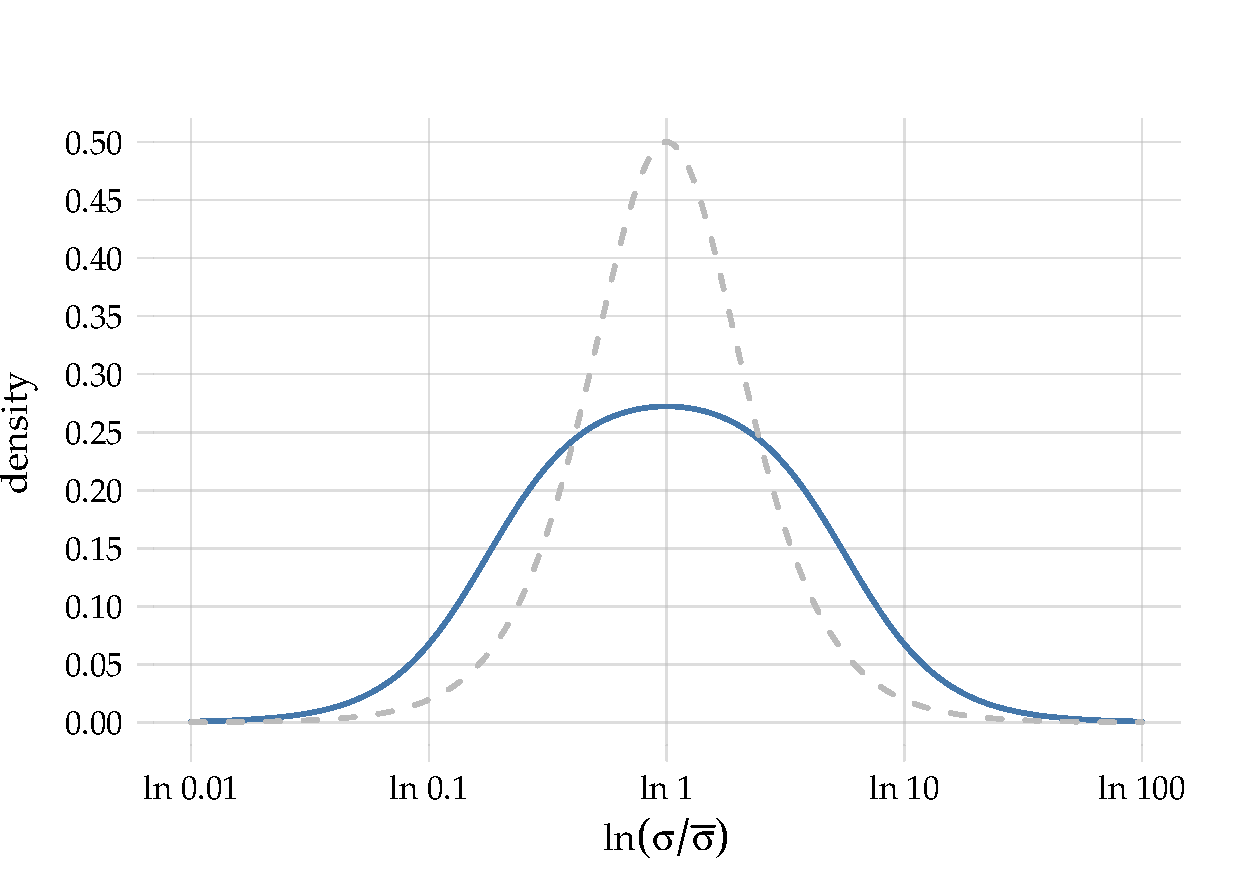
\includegraphics[width=0.75\linewidth]{betaprime.pdf}\\
\caption{Solid blue: equal mixture of beta-prime~\eqref{eq:density_log-sigma}. Dashed grey: unmixed beta-prime with unit shape hyperparameters}\label{fig:betaprime}
\end{figure}

\medskip

The combination of prior densities~\eqref{eq:density_w}, \eqref{eq:density_mu}, \eqref{eq:density_sigma} leads to a distribution $\p(\di F\|I)$ of marginal densities $F(\di x)$, for a real variate $x$, which is illustrated in \fig~\ref{fig:marginal_real}.
%%\setlength{\intextsep}{0ex}% with wrapfigure
%%\setlength{\columnsep}{0ex}% with wrapfigure
\begin{figure}
%\begin{wrapfigure}{r}{0.4\linewidth} % with wrapfigure
\centering
\includegraphics[width=\linewidth]{priorsamples_real.pdf}\\
\caption{399 samples from the density $\p[\di F \| I]$  for the marginal density $F(\di x)$ of a continuous real variate $x$. The vertical grey lines mark the scale $\pm\sigmao$. The thicker green density at the bottom-right corner is the expected marginal density $\E[F(\di x) \| I]$.}\label{fig:marginal_real}
\end{figure}




\medskip



 

% \[ \color{bluepurple}\bm{a} \color{redpurple}\mathbin{\bm{\land}}\color{bluepurple} \bm{b} \]


%%%% examples use empheq
%   \begin{empheq}[left={\mathllap{\begin{aligned}    \de\yF_{\yc}/\de\yp&=0\text{:} \\
%         \de\yF_{\yc}/\de\ym&=0\text{:}\\ \de\yF_{\yc}/\de\yl&=0\text{:}\end{aligned}}\qquad}\empheqlbrace]{align}
%     \label{eq:con_p}
% %    \de\yF_{\yc}/\de\yp &\equiv
%     -\ln\yp + \ln\yq + \yl\yM + \ym\yu &=0,\\
%     \label{eq:con_u}
% %    \de\yF_{\yc}/\de\ym &\equiv
%     \yu\yp-1 &=0,\\
%     \label{eq:con_l}
%     %\de\yF_{\yc}/\de\yl &\equiv
%     \yM\yp-\yc &=0.
%   \end{empheq}
%%%%
% \begin{empheq}[box=\widefbox]{equation}
%   \label{eq:maxent_question}
%   \p\bigl[\yE{N+1}{k} \bigcond \tsum\yo\yf{N}\in\yA, \yM\bigr] = \mathord{?}
% \end{empheq}



% \[
%   \begin{tikzcd}
%       M_{n,n}(\CC) \arrow{r}{R'_{a}(\Hat{U})} & M_{n,n}(\CC)
%     \\
%     L(\mathcal{H}) \arrow{r}{\Hat{U}} \arrow[swap]{d}{R_*}\arrow[swap]{u}{R'_*} & L(\mathcal{H}) \arrow{d}{R_*}\arrow{u}{R'_*} \\
%       M_{n,n}(\CC) \arrow{r}{R_{a}(\Hat{U})} & M_{n,n}(\CC)
%   \end{tikzcd}
% \]

% \[
%   \begin{tikzcd}
%       \CC^n \arrow{r}{R'_*(A)} & \CC^n
%     \\
%     \mathcal{H} \arrow{r}{A} \arrow[swap]{d}{R}\arrow[swap]{u}{R'} & \mathcal{H} \arrow{d}{R}\arrow{u}{R'} \\
%       \CC^n \arrow{r}{R_*(A)} & \CC^n
%   \end{tikzcd}
% \]


% \[
%   \begin{tikzcd}
%     \mathcal{H} \arrow{r}{A} \arrow[swap]{d}{R} & \mathcal{H} \arrow{d}{R} \\
%       \CC^n \arrow{r}{R_*(A)} & \CC^n
%   \end{tikzcd}
% \]

%%\setlength{\intextsep}{0ex}% with wrapfigure
%%\setlength{\columnsep}{0ex}% with wrapfigure
%\begin{figure}[p!]% with figure
%\begin{wrapfigure}{r}{0.4\linewidth} % with wrapfigure
%  \centering\includegraphics[trim={12ex 0 18ex 0},clip,width=\linewidth]{maxent_saddle.png}\\
%\caption{caption}\label{fig:comparison_a5}
%\end{figure}% exp_family_maxent.nb


%%%%%%%%%%%%%%%%%%%%%%%%%%%%%%%%%%%%%%%%%%%%%%%%%%%%%%%%%%%%%%%%%%%%%%%%%%%%
%%% Acknowledgements
%%%%%%%%%%%%%%%%%%%%%%%%%%%%%%%%%%%%%%%%%%%%%%%%%%%%%%%%%%%%%%%%%%%%%%%%%%%% 
\iffalse
\begin{acknowledgements}
  \ldots to Mari \amp\ Miri for continuous encouragement and affection, and
  to Buster Keaton and Saitama for filling life with awe and inspiration.
  To the developers and maintainers of \LaTeX, Emacs, AUC\TeX, Open Science
  Framework, R, Python, Inkscape, Sci-Hub for making a free and impartial
  scientific exchange possible.
  % Our work was supported by the Trond Mohn Research Foundation, grant number BFS2018TMT07
%\rotatebox{15}{P}\rotatebox{5}{I}\rotatebox{-10}{P}\rotatebox{10}{\reflectbox{P}}\rotatebox{-5}{O}.
%\sourceatright{\autanet}
\mbox{}\hfill\autanet
\end{acknowledgements}
\fi

%%%%%%%%%%%%%%%%%%%%%%%%%%%%%%%%%%%%%%%%%%%%%%%%%%%%%%%%%%%%%%%%%%%%%%%%%%%%
%%% Appendices
%%%%%%%%%%%%%%%%%%%%%%%%%%%%%%%%%%%%%%%%%%%%%%%%%%%%%%%%%%%%%%%%%%%%%%%%%%%% 
%\clearpage
\bigskip
% %\renewcommand*{\appendixpagename}{Appendix}
% %\renewcommand*{\appendixname}{Appendix}
% %\appendixpage
% \appendix

%%%%%%%%%%%%%%%%%%%%%%%%%%%%%%%%%%%%%%%%%%%%%%%%%%%%%%%%%%%%%%%%%%%%%%%%%%%%
%%% Bibliography
%%%%%%%%%%%%%%%%%%%%%%%%%%%%%%%%%%%%%%%%%%%%%%%%%%%%%%%%%%%%%%%%%%%%%%%%%%%% 
\renewcommand*{\finalnamedelim}{\addcomma\space}
\defbibnote{prenote}{{\footnotesize (\enquote{de $X$} is listed under D,
    \enquote{van $X$} under V, and so on, regardless of national
    conventions.)\par}}
% \defbibnote{postnote}{\par\medskip\noindent{\footnotesize% Note:
%     \arxivp \mparcp \philscip \biorxivp}}

\printbibliography[prenote=prenote%,postnote=postnote
]

\end{document}

%%%%%%%%%%%%%%%%%%%%%%%%%%%%%%%%%%%%%%%%%%%%%%%%%%%%%%%%%%%%%%%%%%%%%%%%%%%%
%%% Cut text (won't be compiled)
%%%%%%%%%%%%%%%%%%%%%%%%%%%%%%%%%%%%%%%%%%%%%%%%%%%%%%%%%%%%%%%%%%%%%%%%%%%% 


%%% Local Variables: 
%%% mode: LaTeX
%%% TeX-PDF-mode: t
%%% TeX-master: t
%%% End: 
